In this section, the effectiveness of CLIP with prompt engineering for the long-tail issue and AFRICAN for the temporal redundancy problem is experimented with.

\section {Existing Models}
The Animal Kingdom dataset proposed its own model, Collaborative Action Recognition (CARe), for action recognition, which is used as the baseline model in this research. It achieves 30.55\% mAP for all classes, 63.33\% mAP for head classes, 38.62\% mAP for middle classes, and 25.09\% mAP for tail classes. This model is mainly used as the baseline for animal action recognition in this research.

MSQNet \parencite{mondal2023msqnet} was proposed one month before this research and achieved state-of-the-art results on this dataset. To fairly compare MSQNet with AFRICAN proposed in this research, we use the score of MSQNet trained on videos sampled with 8 frames, achieving 67.74\% overall mAP for all classes. 

\section{CLIP with Prompt Engineering}
Before experimentally addressing the long-tail issue, a preliminary decision needs to be made regarding the selection between VideoCLIP and ImageCLIP as the backbone for action recognition. Subsequently, an assessment is conducted to evaluate the effectiveness of CLIP in mitigating the long-tail issue.

\subsection{VideoCLIP or ImageCLIP?}
\label{sec:imageclipbetter}
To make this decision, three model settings are tested: 

\begin{enumerate}
    \item \textbf{VC\_Vision}: VideoCLIP with vision layers learnable, as illustrated in Figure \ref{fig:modelstructure_vc} with a learnable video encoder.
    \item \textbf{VC\_Proj}: VideoCLIP with only projection layers learnable, as illustrated in Figure \ref{fig:modelstructure_vc} with a frozen video encoder.
    \item \textbf{IC}: ImageCLIP trained on post-transformer layers, as illustrated in Figure \ref{fig:modelstructure_ic} with a frozen image encoder.
\end{enumerate}

For all three experiments, the models are trained for 80 epochs on a single A100 GPU using a binary cross-entropy loss function, the adamw optimizer, and a learning rate of 0.00015. The VC\_Vision model employs a batch size of 16 due to memory constraints, while batch sizes of 128 are used for the VC\_Proj and IC models. In accordance with Animal Kingdom settings as referenced from \parencite{ng2022animal}, evaluation metrics for this task include the mean Average Precision (mAP) on the overall, head, middle, and tail classes, as provided by the dataset. 

% TODO
%The effect of batch size for VideoCLIP will be further discussed in Section \ref{sec:discussion_bs}.

The performance on each epoch during the training process is illustrated in Figure \ref{fig:tp_backbone}. As the results are still improving slightly, the performance of the final epoch, Epoch 80, is selected for comparison. 

The results of the three experiments are shown in Table \ref{tab:resultsbackbone}. As illustrated in Figure \ref{fig:tp_backbone}, the IC model significantly outperforms the other two models. Specifically, the VC\_vision model achieves a 27.19\% mAP on the overall dataset, which is the lowest among all experiments. The VC\_Proj model achieves a 49.82\% mAP on the overall dataset, making it the second lowest. In contrast, the IC model achieves a 53.60\% mAP on the overall dataset, the highest among all the other experiments. Although both the IC and VC\_Proj models outperform the baseline model, CARe, which records a 30.55\% mAP on the overall dataset, the IC model surpasses the VC\_Proj model by 3.78\% mAP. Consequently, the IC model is chosen for subsequent experiments. A detailed discussion regarding the performance of ImageCLIP and VideoCLIP can be found in Section \ref{sec:discussion_vc}.

\begin{table}[ht]
    \centering
    \caption[Training Results for Visual Encoder Selection on Epoch 80]{The table shows the training result of VC\_Vision, VC\_Proj, and IC on Epoch 80. \textbf{VC\_Vision} is VideoCLIP with vision layers learnable, as illustrated in Figure \ref{fig:modelstructure_vc} with a learnable video encoder. \textbf{VC\_Proj} is VideoCLIP with only projection layers learnable, as illustrated in Figure \ref{fig:modelstructure_vc} with a frozen video encoder. \textbf{IC} is ImageCLIP trained on post-transformer layers, as illustrated in Figure \ref{fig:modelstructure_ic} with a frozen image encoder.}
    \label{tab:resultsbackbone}
    \begin{tabular}{lllll}
        \toprule
        \multirow{2}{*}{Models} & \multicolumn{4}{c}{mAP (Epoch 80)} \\
        \cmidrule{2-5} 
        {} & Overall & Head  & Middle & Tail \\
        \midrule
        % CARe   \parencite{ng2022animal}     & 30.55   & 63.33 & 38.62 & 25.09 \\
        CARe\parencite{ng2022animal} & 30.55 & \uuline{63.33} & 38.62 & 25.09 \\
        VC\_Vision  & 27.19   & 45.00 & 36.85 & 19.99 \\
        VC\_Proj    & \uuline{49.82} & 59.17 & \uuline{54.93} & \uuline{46.03} \\
        IC          & \textbf{53.60} & \textbf{71.39} & \textbf{59.98} & \textbf{47.58} \\
        \bottomrule
    \end{tabular}
\end{table}

\begin{figure}[ht]
    \centering
    % 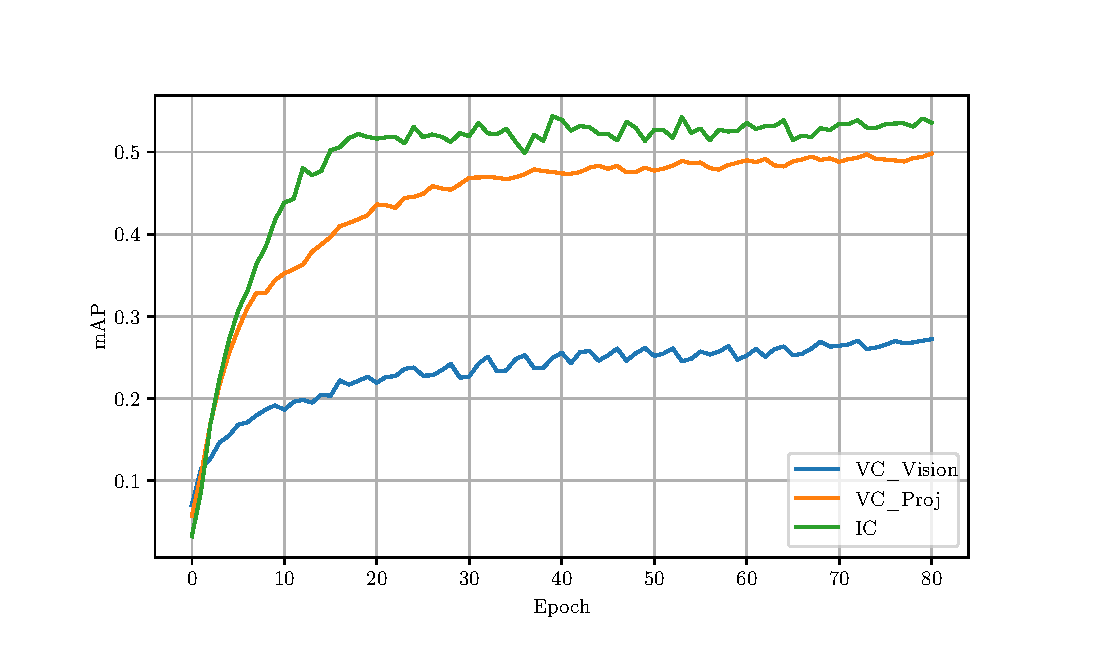
\includegraphics[width=1.0\textwidth]{assets/charts/4_1_BackboneSelection.pgf}
    \resizebox{1.0\textwidth}{!}{%% Creator: Matplotlib, PGF backend
%%
%% To include the figure in your LaTeX document, write
%%   \input{<filename>.pgf}
%%
%% Make sure the required packages are loaded in your preamble
%%   \usepackage{pgf}
%%
%% and, on pdftex
%%   \usepackage[utf8]{inputenc}\DeclareUnicodeCharacter{2212}{-}
%%
%% or, on luatex and xetex
%%   \usepackage{unicode-math}
%%
%% Figures using additional raster images can only be included by \input if
%% they are in the same directory as the main LaTeX file. For loading figures
%% from other directories you can use the `import` package
%%   \usepackage{import}
%%
%% and then include the figures with
%%   \import{<path to file>}{<filename>.pgf}
%%
%% Matplotlib used the following preamble
%%
\begingroup%
\makeatletter%
\begin{pgfpicture}%
\pgfpathrectangle{\pgfpointorigin}{\pgfqpoint{7.000000in}{4.000000in}}%
\pgfusepath{use as bounding box, clip}%
\begin{pgfscope}%
\pgfsetbuttcap%
\pgfsetmiterjoin%
\definecolor{currentfill}{rgb}{1.000000,1.000000,1.000000}%
\pgfsetfillcolor{currentfill}%
\pgfsetlinewidth{0.000000pt}%
\definecolor{currentstroke}{rgb}{1.000000,1.000000,1.000000}%
\pgfsetstrokecolor{currentstroke}%
\pgfsetdash{}{0pt}%
\pgfpathmoveto{\pgfqpoint{0.000000in}{0.000000in}}%
\pgfpathlineto{\pgfqpoint{7.000000in}{0.000000in}}%
\pgfpathlineto{\pgfqpoint{7.000000in}{4.000000in}}%
\pgfpathlineto{\pgfqpoint{0.000000in}{4.000000in}}%
\pgfpathclose%
\pgfusepath{fill}%
\end{pgfscope}%
\begin{pgfscope}%
\pgfsetbuttcap%
\pgfsetmiterjoin%
\definecolor{currentfill}{rgb}{1.000000,1.000000,1.000000}%
\pgfsetfillcolor{currentfill}%
\pgfsetlinewidth{0.000000pt}%
\definecolor{currentstroke}{rgb}{0.000000,0.000000,0.000000}%
\pgfsetstrokecolor{currentstroke}%
\pgfsetstrokeopacity{0.000000}%
\pgfsetdash{}{0pt}%
\pgfpathmoveto{\pgfqpoint{0.875000in}{0.440000in}}%
\pgfpathlineto{\pgfqpoint{6.300000in}{0.440000in}}%
\pgfpathlineto{\pgfqpoint{6.300000in}{3.520000in}}%
\pgfpathlineto{\pgfqpoint{0.875000in}{3.520000in}}%
\pgfpathclose%
\pgfusepath{fill}%
\end{pgfscope}%
\begin{pgfscope}%
\pgfpathrectangle{\pgfqpoint{0.875000in}{0.440000in}}{\pgfqpoint{5.425000in}{3.080000in}}%
\pgfusepath{clip}%
\pgfsetrectcap%
\pgfsetroundjoin%
\pgfsetlinewidth{0.803000pt}%
\definecolor{currentstroke}{rgb}{0.690196,0.690196,0.690196}%
\pgfsetstrokecolor{currentstroke}%
\pgfsetdash{}{0pt}%
\pgfpathmoveto{\pgfqpoint{1.121591in}{0.440000in}}%
\pgfpathlineto{\pgfqpoint{1.121591in}{3.520000in}}%
\pgfusepath{stroke}%
\end{pgfscope}%
\begin{pgfscope}%
\pgfsetbuttcap%
\pgfsetroundjoin%
\definecolor{currentfill}{rgb}{0.000000,0.000000,0.000000}%
\pgfsetfillcolor{currentfill}%
\pgfsetlinewidth{0.803000pt}%
\definecolor{currentstroke}{rgb}{0.000000,0.000000,0.000000}%
\pgfsetstrokecolor{currentstroke}%
\pgfsetdash{}{0pt}%
\pgfsys@defobject{currentmarker}{\pgfqpoint{0.000000in}{-0.048611in}}{\pgfqpoint{0.000000in}{0.000000in}}{%
\pgfpathmoveto{\pgfqpoint{0.000000in}{0.000000in}}%
\pgfpathlineto{\pgfqpoint{0.000000in}{-0.048611in}}%
\pgfusepath{stroke,fill}%
}%
\begin{pgfscope}%
\pgfsys@transformshift{1.121591in}{0.440000in}%
\pgfsys@useobject{currentmarker}{}%
\end{pgfscope}%
\end{pgfscope}%
\begin{pgfscope}%
\definecolor{textcolor}{rgb}{0.000000,0.000000,0.000000}%
\pgfsetstrokecolor{textcolor}%
\pgfsetfillcolor{textcolor}%
\pgftext[x=1.121591in,y=0.342778in,,top]{\color{textcolor}\rmfamily\fontsize{10.000000}{12.000000}\selectfont \(\displaystyle {0}\)}%
\end{pgfscope}%
\begin{pgfscope}%
\pgfpathrectangle{\pgfqpoint{0.875000in}{0.440000in}}{\pgfqpoint{5.425000in}{3.080000in}}%
\pgfusepath{clip}%
\pgfsetrectcap%
\pgfsetroundjoin%
\pgfsetlinewidth{0.803000pt}%
\definecolor{currentstroke}{rgb}{0.690196,0.690196,0.690196}%
\pgfsetstrokecolor{currentstroke}%
\pgfsetdash{}{0pt}%
\pgfpathmoveto{\pgfqpoint{1.738068in}{0.440000in}}%
\pgfpathlineto{\pgfqpoint{1.738068in}{3.520000in}}%
\pgfusepath{stroke}%
\end{pgfscope}%
\begin{pgfscope}%
\pgfsetbuttcap%
\pgfsetroundjoin%
\definecolor{currentfill}{rgb}{0.000000,0.000000,0.000000}%
\pgfsetfillcolor{currentfill}%
\pgfsetlinewidth{0.803000pt}%
\definecolor{currentstroke}{rgb}{0.000000,0.000000,0.000000}%
\pgfsetstrokecolor{currentstroke}%
\pgfsetdash{}{0pt}%
\pgfsys@defobject{currentmarker}{\pgfqpoint{0.000000in}{-0.048611in}}{\pgfqpoint{0.000000in}{0.000000in}}{%
\pgfpathmoveto{\pgfqpoint{0.000000in}{0.000000in}}%
\pgfpathlineto{\pgfqpoint{0.000000in}{-0.048611in}}%
\pgfusepath{stroke,fill}%
}%
\begin{pgfscope}%
\pgfsys@transformshift{1.738068in}{0.440000in}%
\pgfsys@useobject{currentmarker}{}%
\end{pgfscope}%
\end{pgfscope}%
\begin{pgfscope}%
\definecolor{textcolor}{rgb}{0.000000,0.000000,0.000000}%
\pgfsetstrokecolor{textcolor}%
\pgfsetfillcolor{textcolor}%
\pgftext[x=1.738068in,y=0.342778in,,top]{\color{textcolor}\rmfamily\fontsize{10.000000}{12.000000}\selectfont \(\displaystyle {10}\)}%
\end{pgfscope}%
\begin{pgfscope}%
\pgfpathrectangle{\pgfqpoint{0.875000in}{0.440000in}}{\pgfqpoint{5.425000in}{3.080000in}}%
\pgfusepath{clip}%
\pgfsetrectcap%
\pgfsetroundjoin%
\pgfsetlinewidth{0.803000pt}%
\definecolor{currentstroke}{rgb}{0.690196,0.690196,0.690196}%
\pgfsetstrokecolor{currentstroke}%
\pgfsetdash{}{0pt}%
\pgfpathmoveto{\pgfqpoint{2.354545in}{0.440000in}}%
\pgfpathlineto{\pgfqpoint{2.354545in}{3.520000in}}%
\pgfusepath{stroke}%
\end{pgfscope}%
\begin{pgfscope}%
\pgfsetbuttcap%
\pgfsetroundjoin%
\definecolor{currentfill}{rgb}{0.000000,0.000000,0.000000}%
\pgfsetfillcolor{currentfill}%
\pgfsetlinewidth{0.803000pt}%
\definecolor{currentstroke}{rgb}{0.000000,0.000000,0.000000}%
\pgfsetstrokecolor{currentstroke}%
\pgfsetdash{}{0pt}%
\pgfsys@defobject{currentmarker}{\pgfqpoint{0.000000in}{-0.048611in}}{\pgfqpoint{0.000000in}{0.000000in}}{%
\pgfpathmoveto{\pgfqpoint{0.000000in}{0.000000in}}%
\pgfpathlineto{\pgfqpoint{0.000000in}{-0.048611in}}%
\pgfusepath{stroke,fill}%
}%
\begin{pgfscope}%
\pgfsys@transformshift{2.354545in}{0.440000in}%
\pgfsys@useobject{currentmarker}{}%
\end{pgfscope}%
\end{pgfscope}%
\begin{pgfscope}%
\definecolor{textcolor}{rgb}{0.000000,0.000000,0.000000}%
\pgfsetstrokecolor{textcolor}%
\pgfsetfillcolor{textcolor}%
\pgftext[x=2.354545in,y=0.342778in,,top]{\color{textcolor}\rmfamily\fontsize{10.000000}{12.000000}\selectfont \(\displaystyle {20}\)}%
\end{pgfscope}%
\begin{pgfscope}%
\pgfpathrectangle{\pgfqpoint{0.875000in}{0.440000in}}{\pgfqpoint{5.425000in}{3.080000in}}%
\pgfusepath{clip}%
\pgfsetrectcap%
\pgfsetroundjoin%
\pgfsetlinewidth{0.803000pt}%
\definecolor{currentstroke}{rgb}{0.690196,0.690196,0.690196}%
\pgfsetstrokecolor{currentstroke}%
\pgfsetdash{}{0pt}%
\pgfpathmoveto{\pgfqpoint{2.971023in}{0.440000in}}%
\pgfpathlineto{\pgfqpoint{2.971023in}{3.520000in}}%
\pgfusepath{stroke}%
\end{pgfscope}%
\begin{pgfscope}%
\pgfsetbuttcap%
\pgfsetroundjoin%
\definecolor{currentfill}{rgb}{0.000000,0.000000,0.000000}%
\pgfsetfillcolor{currentfill}%
\pgfsetlinewidth{0.803000pt}%
\definecolor{currentstroke}{rgb}{0.000000,0.000000,0.000000}%
\pgfsetstrokecolor{currentstroke}%
\pgfsetdash{}{0pt}%
\pgfsys@defobject{currentmarker}{\pgfqpoint{0.000000in}{-0.048611in}}{\pgfqpoint{0.000000in}{0.000000in}}{%
\pgfpathmoveto{\pgfqpoint{0.000000in}{0.000000in}}%
\pgfpathlineto{\pgfqpoint{0.000000in}{-0.048611in}}%
\pgfusepath{stroke,fill}%
}%
\begin{pgfscope}%
\pgfsys@transformshift{2.971023in}{0.440000in}%
\pgfsys@useobject{currentmarker}{}%
\end{pgfscope}%
\end{pgfscope}%
\begin{pgfscope}%
\definecolor{textcolor}{rgb}{0.000000,0.000000,0.000000}%
\pgfsetstrokecolor{textcolor}%
\pgfsetfillcolor{textcolor}%
\pgftext[x=2.971023in,y=0.342778in,,top]{\color{textcolor}\rmfamily\fontsize{10.000000}{12.000000}\selectfont \(\displaystyle {30}\)}%
\end{pgfscope}%
\begin{pgfscope}%
\pgfpathrectangle{\pgfqpoint{0.875000in}{0.440000in}}{\pgfqpoint{5.425000in}{3.080000in}}%
\pgfusepath{clip}%
\pgfsetrectcap%
\pgfsetroundjoin%
\pgfsetlinewidth{0.803000pt}%
\definecolor{currentstroke}{rgb}{0.690196,0.690196,0.690196}%
\pgfsetstrokecolor{currentstroke}%
\pgfsetdash{}{0pt}%
\pgfpathmoveto{\pgfqpoint{3.587500in}{0.440000in}}%
\pgfpathlineto{\pgfqpoint{3.587500in}{3.520000in}}%
\pgfusepath{stroke}%
\end{pgfscope}%
\begin{pgfscope}%
\pgfsetbuttcap%
\pgfsetroundjoin%
\definecolor{currentfill}{rgb}{0.000000,0.000000,0.000000}%
\pgfsetfillcolor{currentfill}%
\pgfsetlinewidth{0.803000pt}%
\definecolor{currentstroke}{rgb}{0.000000,0.000000,0.000000}%
\pgfsetstrokecolor{currentstroke}%
\pgfsetdash{}{0pt}%
\pgfsys@defobject{currentmarker}{\pgfqpoint{0.000000in}{-0.048611in}}{\pgfqpoint{0.000000in}{0.000000in}}{%
\pgfpathmoveto{\pgfqpoint{0.000000in}{0.000000in}}%
\pgfpathlineto{\pgfqpoint{0.000000in}{-0.048611in}}%
\pgfusepath{stroke,fill}%
}%
\begin{pgfscope}%
\pgfsys@transformshift{3.587500in}{0.440000in}%
\pgfsys@useobject{currentmarker}{}%
\end{pgfscope}%
\end{pgfscope}%
\begin{pgfscope}%
\definecolor{textcolor}{rgb}{0.000000,0.000000,0.000000}%
\pgfsetstrokecolor{textcolor}%
\pgfsetfillcolor{textcolor}%
\pgftext[x=3.587500in,y=0.342778in,,top]{\color{textcolor}\rmfamily\fontsize{10.000000}{12.000000}\selectfont \(\displaystyle {40}\)}%
\end{pgfscope}%
\begin{pgfscope}%
\pgfpathrectangle{\pgfqpoint{0.875000in}{0.440000in}}{\pgfqpoint{5.425000in}{3.080000in}}%
\pgfusepath{clip}%
\pgfsetrectcap%
\pgfsetroundjoin%
\pgfsetlinewidth{0.803000pt}%
\definecolor{currentstroke}{rgb}{0.690196,0.690196,0.690196}%
\pgfsetstrokecolor{currentstroke}%
\pgfsetdash{}{0pt}%
\pgfpathmoveto{\pgfqpoint{4.203977in}{0.440000in}}%
\pgfpathlineto{\pgfqpoint{4.203977in}{3.520000in}}%
\pgfusepath{stroke}%
\end{pgfscope}%
\begin{pgfscope}%
\pgfsetbuttcap%
\pgfsetroundjoin%
\definecolor{currentfill}{rgb}{0.000000,0.000000,0.000000}%
\pgfsetfillcolor{currentfill}%
\pgfsetlinewidth{0.803000pt}%
\definecolor{currentstroke}{rgb}{0.000000,0.000000,0.000000}%
\pgfsetstrokecolor{currentstroke}%
\pgfsetdash{}{0pt}%
\pgfsys@defobject{currentmarker}{\pgfqpoint{0.000000in}{-0.048611in}}{\pgfqpoint{0.000000in}{0.000000in}}{%
\pgfpathmoveto{\pgfqpoint{0.000000in}{0.000000in}}%
\pgfpathlineto{\pgfqpoint{0.000000in}{-0.048611in}}%
\pgfusepath{stroke,fill}%
}%
\begin{pgfscope}%
\pgfsys@transformshift{4.203977in}{0.440000in}%
\pgfsys@useobject{currentmarker}{}%
\end{pgfscope}%
\end{pgfscope}%
\begin{pgfscope}%
\definecolor{textcolor}{rgb}{0.000000,0.000000,0.000000}%
\pgfsetstrokecolor{textcolor}%
\pgfsetfillcolor{textcolor}%
\pgftext[x=4.203977in,y=0.342778in,,top]{\color{textcolor}\rmfamily\fontsize{10.000000}{12.000000}\selectfont \(\displaystyle {50}\)}%
\end{pgfscope}%
\begin{pgfscope}%
\pgfpathrectangle{\pgfqpoint{0.875000in}{0.440000in}}{\pgfqpoint{5.425000in}{3.080000in}}%
\pgfusepath{clip}%
\pgfsetrectcap%
\pgfsetroundjoin%
\pgfsetlinewidth{0.803000pt}%
\definecolor{currentstroke}{rgb}{0.690196,0.690196,0.690196}%
\pgfsetstrokecolor{currentstroke}%
\pgfsetdash{}{0pt}%
\pgfpathmoveto{\pgfqpoint{4.820455in}{0.440000in}}%
\pgfpathlineto{\pgfqpoint{4.820455in}{3.520000in}}%
\pgfusepath{stroke}%
\end{pgfscope}%
\begin{pgfscope}%
\pgfsetbuttcap%
\pgfsetroundjoin%
\definecolor{currentfill}{rgb}{0.000000,0.000000,0.000000}%
\pgfsetfillcolor{currentfill}%
\pgfsetlinewidth{0.803000pt}%
\definecolor{currentstroke}{rgb}{0.000000,0.000000,0.000000}%
\pgfsetstrokecolor{currentstroke}%
\pgfsetdash{}{0pt}%
\pgfsys@defobject{currentmarker}{\pgfqpoint{0.000000in}{-0.048611in}}{\pgfqpoint{0.000000in}{0.000000in}}{%
\pgfpathmoveto{\pgfqpoint{0.000000in}{0.000000in}}%
\pgfpathlineto{\pgfqpoint{0.000000in}{-0.048611in}}%
\pgfusepath{stroke,fill}%
}%
\begin{pgfscope}%
\pgfsys@transformshift{4.820455in}{0.440000in}%
\pgfsys@useobject{currentmarker}{}%
\end{pgfscope}%
\end{pgfscope}%
\begin{pgfscope}%
\definecolor{textcolor}{rgb}{0.000000,0.000000,0.000000}%
\pgfsetstrokecolor{textcolor}%
\pgfsetfillcolor{textcolor}%
\pgftext[x=4.820455in,y=0.342778in,,top]{\color{textcolor}\rmfamily\fontsize{10.000000}{12.000000}\selectfont \(\displaystyle {60}\)}%
\end{pgfscope}%
\begin{pgfscope}%
\pgfpathrectangle{\pgfqpoint{0.875000in}{0.440000in}}{\pgfqpoint{5.425000in}{3.080000in}}%
\pgfusepath{clip}%
\pgfsetrectcap%
\pgfsetroundjoin%
\pgfsetlinewidth{0.803000pt}%
\definecolor{currentstroke}{rgb}{0.690196,0.690196,0.690196}%
\pgfsetstrokecolor{currentstroke}%
\pgfsetdash{}{0pt}%
\pgfpathmoveto{\pgfqpoint{5.436932in}{0.440000in}}%
\pgfpathlineto{\pgfqpoint{5.436932in}{3.520000in}}%
\pgfusepath{stroke}%
\end{pgfscope}%
\begin{pgfscope}%
\pgfsetbuttcap%
\pgfsetroundjoin%
\definecolor{currentfill}{rgb}{0.000000,0.000000,0.000000}%
\pgfsetfillcolor{currentfill}%
\pgfsetlinewidth{0.803000pt}%
\definecolor{currentstroke}{rgb}{0.000000,0.000000,0.000000}%
\pgfsetstrokecolor{currentstroke}%
\pgfsetdash{}{0pt}%
\pgfsys@defobject{currentmarker}{\pgfqpoint{0.000000in}{-0.048611in}}{\pgfqpoint{0.000000in}{0.000000in}}{%
\pgfpathmoveto{\pgfqpoint{0.000000in}{0.000000in}}%
\pgfpathlineto{\pgfqpoint{0.000000in}{-0.048611in}}%
\pgfusepath{stroke,fill}%
}%
\begin{pgfscope}%
\pgfsys@transformshift{5.436932in}{0.440000in}%
\pgfsys@useobject{currentmarker}{}%
\end{pgfscope}%
\end{pgfscope}%
\begin{pgfscope}%
\definecolor{textcolor}{rgb}{0.000000,0.000000,0.000000}%
\pgfsetstrokecolor{textcolor}%
\pgfsetfillcolor{textcolor}%
\pgftext[x=5.436932in,y=0.342778in,,top]{\color{textcolor}\rmfamily\fontsize{10.000000}{12.000000}\selectfont \(\displaystyle {70}\)}%
\end{pgfscope}%
\begin{pgfscope}%
\pgfpathrectangle{\pgfqpoint{0.875000in}{0.440000in}}{\pgfqpoint{5.425000in}{3.080000in}}%
\pgfusepath{clip}%
\pgfsetrectcap%
\pgfsetroundjoin%
\pgfsetlinewidth{0.803000pt}%
\definecolor{currentstroke}{rgb}{0.690196,0.690196,0.690196}%
\pgfsetstrokecolor{currentstroke}%
\pgfsetdash{}{0pt}%
\pgfpathmoveto{\pgfqpoint{6.053409in}{0.440000in}}%
\pgfpathlineto{\pgfqpoint{6.053409in}{3.520000in}}%
\pgfusepath{stroke}%
\end{pgfscope}%
\begin{pgfscope}%
\pgfsetbuttcap%
\pgfsetroundjoin%
\definecolor{currentfill}{rgb}{0.000000,0.000000,0.000000}%
\pgfsetfillcolor{currentfill}%
\pgfsetlinewidth{0.803000pt}%
\definecolor{currentstroke}{rgb}{0.000000,0.000000,0.000000}%
\pgfsetstrokecolor{currentstroke}%
\pgfsetdash{}{0pt}%
\pgfsys@defobject{currentmarker}{\pgfqpoint{0.000000in}{-0.048611in}}{\pgfqpoint{0.000000in}{0.000000in}}{%
\pgfpathmoveto{\pgfqpoint{0.000000in}{0.000000in}}%
\pgfpathlineto{\pgfqpoint{0.000000in}{-0.048611in}}%
\pgfusepath{stroke,fill}%
}%
\begin{pgfscope}%
\pgfsys@transformshift{6.053409in}{0.440000in}%
\pgfsys@useobject{currentmarker}{}%
\end{pgfscope}%
\end{pgfscope}%
\begin{pgfscope}%
\definecolor{textcolor}{rgb}{0.000000,0.000000,0.000000}%
\pgfsetstrokecolor{textcolor}%
\pgfsetfillcolor{textcolor}%
\pgftext[x=6.053409in,y=0.342778in,,top]{\color{textcolor}\rmfamily\fontsize{10.000000}{12.000000}\selectfont \(\displaystyle {80}\)}%
\end{pgfscope}%
\begin{pgfscope}%
\definecolor{textcolor}{rgb}{0.000000,0.000000,0.000000}%
\pgfsetstrokecolor{textcolor}%
\pgfsetfillcolor{textcolor}%
\pgftext[x=3.587500in,y=0.163766in,,top]{\color{textcolor}\rmfamily\fontsize{10.000000}{12.000000}\selectfont Epoch}%
\end{pgfscope}%
\begin{pgfscope}%
\pgfpathrectangle{\pgfqpoint{0.875000in}{0.440000in}}{\pgfqpoint{5.425000in}{3.080000in}}%
\pgfusepath{clip}%
\pgfsetrectcap%
\pgfsetroundjoin%
\pgfsetlinewidth{0.803000pt}%
\definecolor{currentstroke}{rgb}{0.690196,0.690196,0.690196}%
\pgfsetstrokecolor{currentstroke}%
\pgfsetdash{}{0pt}%
\pgfpathmoveto{\pgfqpoint{0.875000in}{0.953310in}}%
\pgfpathlineto{\pgfqpoint{6.300000in}{0.953310in}}%
\pgfusepath{stroke}%
\end{pgfscope}%
\begin{pgfscope}%
\pgfsetbuttcap%
\pgfsetroundjoin%
\definecolor{currentfill}{rgb}{0.000000,0.000000,0.000000}%
\pgfsetfillcolor{currentfill}%
\pgfsetlinewidth{0.803000pt}%
\definecolor{currentstroke}{rgb}{0.000000,0.000000,0.000000}%
\pgfsetstrokecolor{currentstroke}%
\pgfsetdash{}{0pt}%
\pgfsys@defobject{currentmarker}{\pgfqpoint{-0.048611in}{0.000000in}}{\pgfqpoint{0.000000in}{0.000000in}}{%
\pgfpathmoveto{\pgfqpoint{0.000000in}{0.000000in}}%
\pgfpathlineto{\pgfqpoint{-0.048611in}{0.000000in}}%
\pgfusepath{stroke,fill}%
}%
\begin{pgfscope}%
\pgfsys@transformshift{0.875000in}{0.953310in}%
\pgfsys@useobject{currentmarker}{}%
\end{pgfscope}%
\end{pgfscope}%
\begin{pgfscope}%
\definecolor{textcolor}{rgb}{0.000000,0.000000,0.000000}%
\pgfsetstrokecolor{textcolor}%
\pgfsetfillcolor{textcolor}%
\pgftext[x=0.600308in, y=0.905085in, left, base]{\color{textcolor}\rmfamily\fontsize{10.000000}{12.000000}\selectfont \(\displaystyle {0.1}\)}%
\end{pgfscope}%
\begin{pgfscope}%
\pgfpathrectangle{\pgfqpoint{0.875000in}{0.440000in}}{\pgfqpoint{5.425000in}{3.080000in}}%
\pgfusepath{clip}%
\pgfsetrectcap%
\pgfsetroundjoin%
\pgfsetlinewidth{0.803000pt}%
\definecolor{currentstroke}{rgb}{0.690196,0.690196,0.690196}%
\pgfsetstrokecolor{currentstroke}%
\pgfsetdash{}{0pt}%
\pgfpathmoveto{\pgfqpoint{0.875000in}{1.500339in}}%
\pgfpathlineto{\pgfqpoint{6.300000in}{1.500339in}}%
\pgfusepath{stroke}%
\end{pgfscope}%
\begin{pgfscope}%
\pgfsetbuttcap%
\pgfsetroundjoin%
\definecolor{currentfill}{rgb}{0.000000,0.000000,0.000000}%
\pgfsetfillcolor{currentfill}%
\pgfsetlinewidth{0.803000pt}%
\definecolor{currentstroke}{rgb}{0.000000,0.000000,0.000000}%
\pgfsetstrokecolor{currentstroke}%
\pgfsetdash{}{0pt}%
\pgfsys@defobject{currentmarker}{\pgfqpoint{-0.048611in}{0.000000in}}{\pgfqpoint{0.000000in}{0.000000in}}{%
\pgfpathmoveto{\pgfqpoint{0.000000in}{0.000000in}}%
\pgfpathlineto{\pgfqpoint{-0.048611in}{0.000000in}}%
\pgfusepath{stroke,fill}%
}%
\begin{pgfscope}%
\pgfsys@transformshift{0.875000in}{1.500339in}%
\pgfsys@useobject{currentmarker}{}%
\end{pgfscope}%
\end{pgfscope}%
\begin{pgfscope}%
\definecolor{textcolor}{rgb}{0.000000,0.000000,0.000000}%
\pgfsetstrokecolor{textcolor}%
\pgfsetfillcolor{textcolor}%
\pgftext[x=0.600308in, y=1.452113in, left, base]{\color{textcolor}\rmfamily\fontsize{10.000000}{12.000000}\selectfont \(\displaystyle {0.2}\)}%
\end{pgfscope}%
\begin{pgfscope}%
\pgfpathrectangle{\pgfqpoint{0.875000in}{0.440000in}}{\pgfqpoint{5.425000in}{3.080000in}}%
\pgfusepath{clip}%
\pgfsetrectcap%
\pgfsetroundjoin%
\pgfsetlinewidth{0.803000pt}%
\definecolor{currentstroke}{rgb}{0.690196,0.690196,0.690196}%
\pgfsetstrokecolor{currentstroke}%
\pgfsetdash{}{0pt}%
\pgfpathmoveto{\pgfqpoint{0.875000in}{2.047367in}}%
\pgfpathlineto{\pgfqpoint{6.300000in}{2.047367in}}%
\pgfusepath{stroke}%
\end{pgfscope}%
\begin{pgfscope}%
\pgfsetbuttcap%
\pgfsetroundjoin%
\definecolor{currentfill}{rgb}{0.000000,0.000000,0.000000}%
\pgfsetfillcolor{currentfill}%
\pgfsetlinewidth{0.803000pt}%
\definecolor{currentstroke}{rgb}{0.000000,0.000000,0.000000}%
\pgfsetstrokecolor{currentstroke}%
\pgfsetdash{}{0pt}%
\pgfsys@defobject{currentmarker}{\pgfqpoint{-0.048611in}{0.000000in}}{\pgfqpoint{0.000000in}{0.000000in}}{%
\pgfpathmoveto{\pgfqpoint{0.000000in}{0.000000in}}%
\pgfpathlineto{\pgfqpoint{-0.048611in}{0.000000in}}%
\pgfusepath{stroke,fill}%
}%
\begin{pgfscope}%
\pgfsys@transformshift{0.875000in}{2.047367in}%
\pgfsys@useobject{currentmarker}{}%
\end{pgfscope}%
\end{pgfscope}%
\begin{pgfscope}%
\definecolor{textcolor}{rgb}{0.000000,0.000000,0.000000}%
\pgfsetstrokecolor{textcolor}%
\pgfsetfillcolor{textcolor}%
\pgftext[x=0.600308in, y=1.999141in, left, base]{\color{textcolor}\rmfamily\fontsize{10.000000}{12.000000}\selectfont \(\displaystyle {0.3}\)}%
\end{pgfscope}%
\begin{pgfscope}%
\pgfpathrectangle{\pgfqpoint{0.875000in}{0.440000in}}{\pgfqpoint{5.425000in}{3.080000in}}%
\pgfusepath{clip}%
\pgfsetrectcap%
\pgfsetroundjoin%
\pgfsetlinewidth{0.803000pt}%
\definecolor{currentstroke}{rgb}{0.690196,0.690196,0.690196}%
\pgfsetstrokecolor{currentstroke}%
\pgfsetdash{}{0pt}%
\pgfpathmoveto{\pgfqpoint{0.875000in}{2.594395in}}%
\pgfpathlineto{\pgfqpoint{6.300000in}{2.594395in}}%
\pgfusepath{stroke}%
\end{pgfscope}%
\begin{pgfscope}%
\pgfsetbuttcap%
\pgfsetroundjoin%
\definecolor{currentfill}{rgb}{0.000000,0.000000,0.000000}%
\pgfsetfillcolor{currentfill}%
\pgfsetlinewidth{0.803000pt}%
\definecolor{currentstroke}{rgb}{0.000000,0.000000,0.000000}%
\pgfsetstrokecolor{currentstroke}%
\pgfsetdash{}{0pt}%
\pgfsys@defobject{currentmarker}{\pgfqpoint{-0.048611in}{0.000000in}}{\pgfqpoint{0.000000in}{0.000000in}}{%
\pgfpathmoveto{\pgfqpoint{0.000000in}{0.000000in}}%
\pgfpathlineto{\pgfqpoint{-0.048611in}{0.000000in}}%
\pgfusepath{stroke,fill}%
}%
\begin{pgfscope}%
\pgfsys@transformshift{0.875000in}{2.594395in}%
\pgfsys@useobject{currentmarker}{}%
\end{pgfscope}%
\end{pgfscope}%
\begin{pgfscope}%
\definecolor{textcolor}{rgb}{0.000000,0.000000,0.000000}%
\pgfsetstrokecolor{textcolor}%
\pgfsetfillcolor{textcolor}%
\pgftext[x=0.600308in, y=2.546170in, left, base]{\color{textcolor}\rmfamily\fontsize{10.000000}{12.000000}\selectfont \(\displaystyle {0.4}\)}%
\end{pgfscope}%
\begin{pgfscope}%
\pgfpathrectangle{\pgfqpoint{0.875000in}{0.440000in}}{\pgfqpoint{5.425000in}{3.080000in}}%
\pgfusepath{clip}%
\pgfsetrectcap%
\pgfsetroundjoin%
\pgfsetlinewidth{0.803000pt}%
\definecolor{currentstroke}{rgb}{0.690196,0.690196,0.690196}%
\pgfsetstrokecolor{currentstroke}%
\pgfsetdash{}{0pt}%
\pgfpathmoveto{\pgfqpoint{0.875000in}{3.141423in}}%
\pgfpathlineto{\pgfqpoint{6.300000in}{3.141423in}}%
\pgfusepath{stroke}%
\end{pgfscope}%
\begin{pgfscope}%
\pgfsetbuttcap%
\pgfsetroundjoin%
\definecolor{currentfill}{rgb}{0.000000,0.000000,0.000000}%
\pgfsetfillcolor{currentfill}%
\pgfsetlinewidth{0.803000pt}%
\definecolor{currentstroke}{rgb}{0.000000,0.000000,0.000000}%
\pgfsetstrokecolor{currentstroke}%
\pgfsetdash{}{0pt}%
\pgfsys@defobject{currentmarker}{\pgfqpoint{-0.048611in}{0.000000in}}{\pgfqpoint{0.000000in}{0.000000in}}{%
\pgfpathmoveto{\pgfqpoint{0.000000in}{0.000000in}}%
\pgfpathlineto{\pgfqpoint{-0.048611in}{0.000000in}}%
\pgfusepath{stroke,fill}%
}%
\begin{pgfscope}%
\pgfsys@transformshift{0.875000in}{3.141423in}%
\pgfsys@useobject{currentmarker}{}%
\end{pgfscope}%
\end{pgfscope}%
\begin{pgfscope}%
\definecolor{textcolor}{rgb}{0.000000,0.000000,0.000000}%
\pgfsetstrokecolor{textcolor}%
\pgfsetfillcolor{textcolor}%
\pgftext[x=0.600308in, y=3.093198in, left, base]{\color{textcolor}\rmfamily\fontsize{10.000000}{12.000000}\selectfont \(\displaystyle {0.5}\)}%
\end{pgfscope}%
\begin{pgfscope}%
\definecolor{textcolor}{rgb}{0.000000,0.000000,0.000000}%
\pgfsetstrokecolor{textcolor}%
\pgfsetfillcolor{textcolor}%
\pgftext[x=0.544752in,y=1.980000in,,bottom,rotate=90.000000]{\color{textcolor}\rmfamily\fontsize{10.000000}{12.000000}\selectfont mAP}%
\end{pgfscope}%
\begin{pgfscope}%
\pgfpathrectangle{\pgfqpoint{0.875000in}{0.440000in}}{\pgfqpoint{5.425000in}{3.080000in}}%
\pgfusepath{clip}%
\pgfsetrectcap%
\pgfsetroundjoin%
\pgfsetlinewidth{1.505625pt}%
\definecolor{currentstroke}{rgb}{0.121569,0.466667,0.705882}%
\pgfsetstrokecolor{currentstroke}%
\pgfsetdash{}{0pt}%
\pgfpathmoveto{\pgfqpoint{1.121591in}{0.790032in}}%
\pgfpathlineto{\pgfqpoint{1.183239in}{1.031670in}}%
\pgfpathlineto{\pgfqpoint{1.244886in}{1.097626in}}%
\pgfpathlineto{\pgfqpoint{1.306534in}{1.206504in}}%
\pgfpathlineto{\pgfqpoint{1.368182in}{1.250288in}}%
\pgfpathlineto{\pgfqpoint{1.429830in}{1.323820in}}%
\pgfpathlineto{\pgfqpoint{1.491477in}{1.340464in}}%
\pgfpathlineto{\pgfqpoint{1.553125in}{1.387178in}}%
\pgfpathlineto{\pgfqpoint{1.614773in}{1.425803in}}%
\pgfpathlineto{\pgfqpoint{1.676420in}{1.453569in}}%
\pgfpathlineto{\pgfqpoint{1.738068in}{1.423318in}}%
\pgfpathlineto{\pgfqpoint{1.799716in}{1.476685in}}%
\pgfpathlineto{\pgfqpoint{1.861364in}{1.489150in}}%
\pgfpathlineto{\pgfqpoint{1.923011in}{1.471761in}}%
\pgfpathlineto{\pgfqpoint{1.984659in}{1.525217in}}%
\pgfpathlineto{\pgfqpoint{2.046307in}{1.516235in}}%
\pgfpathlineto{\pgfqpoint{2.107955in}{1.619298in}}%
\pgfpathlineto{\pgfqpoint{2.169602in}{1.591322in}}%
\pgfpathlineto{\pgfqpoint{2.231250in}{1.616672in}}%
\pgfpathlineto{\pgfqpoint{2.292898in}{1.644373in}}%
\pgfpathlineto{\pgfqpoint{2.354545in}{1.603481in}}%
\pgfpathlineto{\pgfqpoint{2.416193in}{1.643884in}}%
\pgfpathlineto{\pgfqpoint{2.477841in}{1.647356in}}%
\pgfpathlineto{\pgfqpoint{2.539489in}{1.696610in}}%
\pgfpathlineto{\pgfqpoint{2.601136in}{1.705648in}}%
\pgfpathlineto{\pgfqpoint{2.662784in}{1.651535in}}%
\pgfpathlineto{\pgfqpoint{2.724432in}{1.653559in}}%
\pgfpathlineto{\pgfqpoint{2.786080in}{1.687076in}}%
\pgfpathlineto{\pgfqpoint{2.847727in}{1.729877in}}%
\pgfpathlineto{\pgfqpoint{2.909375in}{1.636803in}}%
\pgfpathlineto{\pgfqpoint{2.971023in}{1.646038in}}%
\pgfpathlineto{\pgfqpoint{3.032670in}{1.731818in}}%
\pgfpathlineto{\pgfqpoint{3.094318in}{1.778419in}}%
\pgfpathlineto{\pgfqpoint{3.155966in}{1.680050in}}%
\pgfpathlineto{\pgfqpoint{3.217614in}{1.686401in}}%
\pgfpathlineto{\pgfqpoint{3.279261in}{1.760793in}}%
\pgfpathlineto{\pgfqpoint{3.340909in}{1.788454in}}%
\pgfpathlineto{\pgfqpoint{3.402557in}{1.702096in}}%
\pgfpathlineto{\pgfqpoint{3.464205in}{1.702846in}}%
\pgfpathlineto{\pgfqpoint{3.525852in}{1.770005in}}%
\pgfpathlineto{\pgfqpoint{3.587500in}{1.804481in}}%
\pgfpathlineto{\pgfqpoint{3.649148in}{1.734448in}}%
\pgfpathlineto{\pgfqpoint{3.710795in}{1.810009in}}%
\pgfpathlineto{\pgfqpoint{3.772443in}{1.814459in}}%
\pgfpathlineto{\pgfqpoint{3.834091in}{1.751825in}}%
\pgfpathlineto{\pgfqpoint{3.895739in}{1.787175in}}%
\pgfpathlineto{\pgfqpoint{3.957386in}{1.832313in}}%
\pgfpathlineto{\pgfqpoint{4.019034in}{1.750698in}}%
\pgfpathlineto{\pgfqpoint{4.080682in}{1.800504in}}%
\pgfpathlineto{\pgfqpoint{4.142330in}{1.835156in}}%
\pgfpathlineto{\pgfqpoint{4.203977in}{1.782828in}}%
\pgfpathlineto{\pgfqpoint{4.265625in}{1.798918in}}%
\pgfpathlineto{\pgfqpoint{4.327273in}{1.832474in}}%
\pgfpathlineto{\pgfqpoint{4.388920in}{1.747442in}}%
\pgfpathlineto{\pgfqpoint{4.450568in}{1.763836in}}%
\pgfpathlineto{\pgfqpoint{4.512216in}{1.812448in}}%
\pgfpathlineto{\pgfqpoint{4.573864in}{1.792438in}}%
\pgfpathlineto{\pgfqpoint{4.635511in}{1.811624in}}%
\pgfpathlineto{\pgfqpoint{4.697159in}{1.848257in}}%
\pgfpathlineto{\pgfqpoint{4.758807in}{1.758893in}}%
\pgfpathlineto{\pgfqpoint{4.820455in}{1.784099in}}%
\pgfpathlineto{\pgfqpoint{4.882102in}{1.830472in}}%
\pgfpathlineto{\pgfqpoint{4.943750in}{1.777703in}}%
\pgfpathlineto{\pgfqpoint{5.005398in}{1.828534in}}%
\pgfpathlineto{\pgfqpoint{5.067045in}{1.845709in}}%
\pgfpathlineto{\pgfqpoint{5.128693in}{1.786853in}}%
\pgfpathlineto{\pgfqpoint{5.190341in}{1.797833in}}%
\pgfpathlineto{\pgfqpoint{5.251989in}{1.831889in}}%
\pgfpathlineto{\pgfqpoint{5.313636in}{1.878756in}}%
\pgfpathlineto{\pgfqpoint{5.375284in}{1.844882in}}%
\pgfpathlineto{\pgfqpoint{5.436932in}{1.850491in}}%
\pgfpathlineto{\pgfqpoint{5.498580in}{1.859866in}}%
\pgfpathlineto{\pgfqpoint{5.560227in}{1.885211in}}%
\pgfpathlineto{\pgfqpoint{5.621875in}{1.828183in}}%
\pgfpathlineto{\pgfqpoint{5.683523in}{1.839448in}}%
\pgfpathlineto{\pgfqpoint{5.745170in}{1.856508in}}%
\pgfpathlineto{\pgfqpoint{5.806818in}{1.882086in}}%
\pgfpathlineto{\pgfqpoint{5.868466in}{1.868961in}}%
\pgfpathlineto{\pgfqpoint{5.930114in}{1.872544in}}%
\pgfpathlineto{\pgfqpoint{5.991761in}{1.884158in}}%
\pgfpathlineto{\pgfqpoint{6.053409in}{1.893860in}}%
\pgfusepath{stroke}%
\end{pgfscope}%
\begin{pgfscope}%
\pgfpathrectangle{\pgfqpoint{0.875000in}{0.440000in}}{\pgfqpoint{5.425000in}{3.080000in}}%
\pgfusepath{clip}%
\pgfsetrectcap%
\pgfsetroundjoin%
\pgfsetlinewidth{1.505625pt}%
\definecolor{currentstroke}{rgb}{1.000000,0.498039,0.054902}%
\pgfsetstrokecolor{currentstroke}%
\pgfsetdash{}{0pt}%
\pgfpathmoveto{\pgfqpoint{1.121591in}{0.714849in}}%
\pgfpathlineto{\pgfqpoint{1.183239in}{0.992165in}}%
\pgfpathlineto{\pgfqpoint{1.244886in}{1.330939in}}%
\pgfpathlineto{\pgfqpoint{1.306534in}{1.589807in}}%
\pgfpathlineto{\pgfqpoint{1.368182in}{1.797751in}}%
\pgfpathlineto{\pgfqpoint{1.429830in}{1.958740in}}%
\pgfpathlineto{\pgfqpoint{1.491477in}{2.101107in}}%
\pgfpathlineto{\pgfqpoint{1.553125in}{2.204821in}}%
\pgfpathlineto{\pgfqpoint{1.614773in}{2.204202in}}%
\pgfpathlineto{\pgfqpoint{1.676420in}{2.288250in}}%
\pgfpathlineto{\pgfqpoint{1.738068in}{2.332916in}}%
\pgfpathlineto{\pgfqpoint{1.799716in}{2.360617in}}%
\pgfpathlineto{\pgfqpoint{1.861364in}{2.390491in}}%
\pgfpathlineto{\pgfqpoint{1.923011in}{2.477837in}}%
\pgfpathlineto{\pgfqpoint{1.984659in}{2.526460in}}%
\pgfpathlineto{\pgfqpoint{2.046307in}{2.575560in}}%
\pgfpathlineto{\pgfqpoint{2.107955in}{2.647701in}}%
\pgfpathlineto{\pgfqpoint{2.169602in}{2.669460in}}%
\pgfpathlineto{\pgfqpoint{2.231250in}{2.694414in}}%
\pgfpathlineto{\pgfqpoint{2.292898in}{2.721231in}}%
\pgfpathlineto{\pgfqpoint{2.354545in}{2.793201in}}%
\pgfpathlineto{\pgfqpoint{2.416193in}{2.787920in}}%
\pgfpathlineto{\pgfqpoint{2.477841in}{2.770472in}}%
\pgfpathlineto{\pgfqpoint{2.539489in}{2.836101in}}%
\pgfpathlineto{\pgfqpoint{2.601136in}{2.844136in}}%
\pgfpathlineto{\pgfqpoint{2.662784in}{2.863048in}}%
\pgfpathlineto{\pgfqpoint{2.724432in}{2.914538in}}%
\pgfpathlineto{\pgfqpoint{2.786080in}{2.899724in}}%
\pgfpathlineto{\pgfqpoint{2.847727in}{2.890382in}}%
\pgfpathlineto{\pgfqpoint{2.909375in}{2.928009in}}%
\pgfpathlineto{\pgfqpoint{2.971023in}{2.971903in}}%
\pgfpathlineto{\pgfqpoint{3.032670in}{2.972192in}}%
\pgfpathlineto{\pgfqpoint{3.094318in}{2.975101in}}%
\pgfpathlineto{\pgfqpoint{3.155966in}{2.971218in}}%
\pgfpathlineto{\pgfqpoint{3.217614in}{2.960328in}}%
\pgfpathlineto{\pgfqpoint{3.279261in}{2.974473in}}%
\pgfpathlineto{\pgfqpoint{3.340909in}{2.993257in}}%
\pgfpathlineto{\pgfqpoint{3.402557in}{3.027632in}}%
\pgfpathlineto{\pgfqpoint{3.464205in}{3.014936in}}%
\pgfpathlineto{\pgfqpoint{3.525852in}{3.009781in}}%
\pgfpathlineto{\pgfqpoint{3.587500in}{2.999169in}}%
\pgfpathlineto{\pgfqpoint{3.649148in}{2.997763in}}%
\pgfpathlineto{\pgfqpoint{3.710795in}{3.008670in}}%
\pgfpathlineto{\pgfqpoint{3.772443in}{3.038637in}}%
\pgfpathlineto{\pgfqpoint{3.834091in}{3.051516in}}%
\pgfpathlineto{\pgfqpoint{3.895739in}{3.030128in}}%
\pgfpathlineto{\pgfqpoint{3.957386in}{3.049796in}}%
\pgfpathlineto{\pgfqpoint{4.019034in}{3.006330in}}%
\pgfpathlineto{\pgfqpoint{4.080682in}{3.006665in}}%
\pgfpathlineto{\pgfqpoint{4.142330in}{3.038056in}}%
\pgfpathlineto{\pgfqpoint{4.203977in}{3.017741in}}%
\pgfpathlineto{\pgfqpoint{4.265625in}{3.032005in}}%
\pgfpathlineto{\pgfqpoint{4.327273in}{3.051451in}}%
\pgfpathlineto{\pgfqpoint{4.388920in}{3.083641in}}%
\pgfpathlineto{\pgfqpoint{4.450568in}{3.066788in}}%
\pgfpathlineto{\pgfqpoint{4.512216in}{3.072402in}}%
\pgfpathlineto{\pgfqpoint{4.573864in}{3.034949in}}%
\pgfpathlineto{\pgfqpoint{4.635511in}{3.024415in}}%
\pgfpathlineto{\pgfqpoint{4.697159in}{3.055287in}}%
\pgfpathlineto{\pgfqpoint{4.758807in}{3.070780in}}%
\pgfpathlineto{\pgfqpoint{4.820455in}{3.087380in}}%
\pgfpathlineto{\pgfqpoint{4.882102in}{3.074728in}}%
\pgfpathlineto{\pgfqpoint{4.943750in}{3.096574in}}%
\pgfpathlineto{\pgfqpoint{5.005398in}{3.053324in}}%
\pgfpathlineto{\pgfqpoint{5.067045in}{3.045811in}}%
\pgfpathlineto{\pgfqpoint{5.128693in}{3.079518in}}%
\pgfpathlineto{\pgfqpoint{5.190341in}{3.092906in}}%
\pgfpathlineto{\pgfqpoint{5.251989in}{3.111983in}}%
\pgfpathlineto{\pgfqpoint{5.313636in}{3.089045in}}%
\pgfpathlineto{\pgfqpoint{5.375284in}{3.100466in}}%
\pgfpathlineto{\pgfqpoint{5.436932in}{3.076536in}}%
\pgfpathlineto{\pgfqpoint{5.498580in}{3.095153in}}%
\pgfpathlineto{\pgfqpoint{5.560227in}{3.104125in}}%
\pgfpathlineto{\pgfqpoint{5.621875in}{3.127562in}}%
\pgfpathlineto{\pgfqpoint{5.683523in}{3.094836in}}%
\pgfpathlineto{\pgfqpoint{5.745170in}{3.092275in}}%
\pgfpathlineto{\pgfqpoint{5.806818in}{3.086400in}}%
\pgfpathlineto{\pgfqpoint{5.868466in}{3.079059in}}%
\pgfpathlineto{\pgfqpoint{5.930114in}{3.100980in}}%
\pgfpathlineto{\pgfqpoint{5.991761in}{3.109960in}}%
\pgfpathlineto{\pgfqpoint{6.053409in}{3.131524in}}%
\pgfusepath{stroke}%
\end{pgfscope}%
\begin{pgfscope}%
\pgfpathrectangle{\pgfqpoint{0.875000in}{0.440000in}}{\pgfqpoint{5.425000in}{3.080000in}}%
\pgfusepath{clip}%
\pgfsetrectcap%
\pgfsetroundjoin%
\pgfsetlinewidth{1.505625pt}%
\definecolor{currentstroke}{rgb}{0.172549,0.627451,0.172549}%
\pgfsetstrokecolor{currentstroke}%
\pgfsetdash{}{0pt}%
\pgfpathmoveto{\pgfqpoint{1.121591in}{0.580000in}}%
\pgfpathlineto{\pgfqpoint{1.183239in}{0.881571in}}%
\pgfpathlineto{\pgfqpoint{1.244886in}{1.327626in}}%
\pgfpathlineto{\pgfqpoint{1.306534in}{1.631724in}}%
\pgfpathlineto{\pgfqpoint{1.368182in}{1.886363in}}%
\pgfpathlineto{\pgfqpoint{1.429830in}{2.084715in}}%
\pgfpathlineto{\pgfqpoint{1.491477in}{2.215711in}}%
\pgfpathlineto{\pgfqpoint{1.553125in}{2.395821in}}%
\pgfpathlineto{\pgfqpoint{1.614773in}{2.513427in}}%
\pgfpathlineto{\pgfqpoint{1.676420in}{2.689845in}}%
\pgfpathlineto{\pgfqpoint{1.738068in}{2.805213in}}%
\pgfpathlineto{\pgfqpoint{1.799716in}{2.829087in}}%
\pgfpathlineto{\pgfqpoint{1.861364in}{3.034721in}}%
\pgfpathlineto{\pgfqpoint{1.923011in}{2.988279in}}%
\pgfpathlineto{\pgfqpoint{1.984659in}{3.015309in}}%
\pgfpathlineto{\pgfqpoint{2.046307in}{3.154835in}}%
\pgfpathlineto{\pgfqpoint{2.107955in}{3.174444in}}%
\pgfpathlineto{\pgfqpoint{2.169602in}{3.235771in}}%
\pgfpathlineto{\pgfqpoint{2.231250in}{3.262258in}}%
\pgfpathlineto{\pgfqpoint{2.292898in}{3.243285in}}%
\pgfpathlineto{\pgfqpoint{2.354545in}{3.231564in}}%
\pgfpathlineto{\pgfqpoint{2.416193in}{3.240098in}}%
\pgfpathlineto{\pgfqpoint{2.477841in}{3.242889in}}%
\pgfpathlineto{\pgfqpoint{2.539489in}{3.200197in}}%
\pgfpathlineto{\pgfqpoint{2.601136in}{3.309805in}}%
\pgfpathlineto{\pgfqpoint{2.662784in}{3.241657in}}%
\pgfpathlineto{\pgfqpoint{2.724432in}{3.259529in}}%
\pgfpathlineto{\pgfqpoint{2.786080in}{3.244035in}}%
\pgfpathlineto{\pgfqpoint{2.847727in}{3.210026in}}%
\pgfpathlineto{\pgfqpoint{2.909375in}{3.268934in}}%
\pgfpathlineto{\pgfqpoint{2.971023in}{3.247863in}}%
\pgfpathlineto{\pgfqpoint{3.032670in}{3.336908in}}%
\pgfpathlineto{\pgfqpoint{3.094318in}{3.267038in}}%
\pgfpathlineto{\pgfqpoint{3.155966in}{3.260343in}}%
\pgfpathlineto{\pgfqpoint{3.217614in}{3.298804in}}%
\pgfpathlineto{\pgfqpoint{3.279261in}{3.210063in}}%
\pgfpathlineto{\pgfqpoint{3.340909in}{3.135896in}}%
\pgfpathlineto{\pgfqpoint{3.402557in}{3.257195in}}%
\pgfpathlineto{\pgfqpoint{3.464205in}{3.216322in}}%
\pgfpathlineto{\pgfqpoint{3.525852in}{3.380000in}}%
\pgfpathlineto{\pgfqpoint{3.587500in}{3.357641in}}%
\pgfpathlineto{\pgfqpoint{3.649148in}{3.285265in}}%
\pgfpathlineto{\pgfqpoint{3.710795in}{3.315143in}}%
\pgfpathlineto{\pgfqpoint{3.772443in}{3.307537in}}%
\pgfpathlineto{\pgfqpoint{3.834091in}{3.263739in}}%
\pgfpathlineto{\pgfqpoint{3.895739in}{3.261992in}}%
\pgfpathlineto{\pgfqpoint{3.957386in}{3.219693in}}%
\pgfpathlineto{\pgfqpoint{4.019034in}{3.345282in}}%
\pgfpathlineto{\pgfqpoint{4.080682in}{3.304350in}}%
\pgfpathlineto{\pgfqpoint{4.142330in}{3.216591in}}%
\pgfpathlineto{\pgfqpoint{4.203977in}{3.289542in}}%
\pgfpathlineto{\pgfqpoint{4.265625in}{3.289866in}}%
\pgfpathlineto{\pgfqpoint{4.327273in}{3.236729in}}%
\pgfpathlineto{\pgfqpoint{4.388920in}{3.374818in}}%
\pgfpathlineto{\pgfqpoint{4.450568in}{3.270997in}}%
\pgfpathlineto{\pgfqpoint{4.512216in}{3.298809in}}%
\pgfpathlineto{\pgfqpoint{4.573864in}{3.220866in}}%
\pgfpathlineto{\pgfqpoint{4.635511in}{3.290807in}}%
\pgfpathlineto{\pgfqpoint{4.697159in}{3.278629in}}%
\pgfpathlineto{\pgfqpoint{4.758807in}{3.284128in}}%
\pgfpathlineto{\pgfqpoint{4.820455in}{3.337202in}}%
\pgfpathlineto{\pgfqpoint{4.882102in}{3.296024in}}%
\pgfpathlineto{\pgfqpoint{4.943750in}{3.315402in}}%
\pgfpathlineto{\pgfqpoint{5.005398in}{3.315180in}}%
\pgfpathlineto{\pgfqpoint{5.067045in}{3.353918in}}%
\pgfpathlineto{\pgfqpoint{5.128693in}{3.221495in}}%
\pgfpathlineto{\pgfqpoint{5.190341in}{3.252137in}}%
\pgfpathlineto{\pgfqpoint{5.251989in}{3.241057in}}%
\pgfpathlineto{\pgfqpoint{5.313636in}{3.301537in}}%
\pgfpathlineto{\pgfqpoint{5.375284in}{3.288710in}}%
\pgfpathlineto{\pgfqpoint{5.436932in}{3.330551in}}%
\pgfpathlineto{\pgfqpoint{5.498580in}{3.329393in}}%
\pgfpathlineto{\pgfqpoint{5.560227in}{3.354535in}}%
\pgfpathlineto{\pgfqpoint{5.621875in}{3.305444in}}%
\pgfpathlineto{\pgfqpoint{5.683523in}{3.303672in}}%
\pgfpathlineto{\pgfqpoint{5.745170in}{3.326910in}}%
\pgfpathlineto{\pgfqpoint{5.806818in}{3.332522in}}%
\pgfpathlineto{\pgfqpoint{5.868466in}{3.333571in}}%
\pgfpathlineto{\pgfqpoint{5.930114in}{3.311190in}}%
\pgfpathlineto{\pgfqpoint{5.991761in}{3.365594in}}%
\pgfpathlineto{\pgfqpoint{6.053409in}{3.338450in}}%
\pgfusepath{stroke}%
\end{pgfscope}%
\begin{pgfscope}%
\pgfsetrectcap%
\pgfsetmiterjoin%
\pgfsetlinewidth{0.803000pt}%
\definecolor{currentstroke}{rgb}{0.000000,0.000000,0.000000}%
\pgfsetstrokecolor{currentstroke}%
\pgfsetdash{}{0pt}%
\pgfpathmoveto{\pgfqpoint{0.875000in}{0.440000in}}%
\pgfpathlineto{\pgfqpoint{0.875000in}{3.520000in}}%
\pgfusepath{stroke}%
\end{pgfscope}%
\begin{pgfscope}%
\pgfsetrectcap%
\pgfsetmiterjoin%
\pgfsetlinewidth{0.803000pt}%
\definecolor{currentstroke}{rgb}{0.000000,0.000000,0.000000}%
\pgfsetstrokecolor{currentstroke}%
\pgfsetdash{}{0pt}%
\pgfpathmoveto{\pgfqpoint{6.300000in}{0.440000in}}%
\pgfpathlineto{\pgfqpoint{6.300000in}{3.520000in}}%
\pgfusepath{stroke}%
\end{pgfscope}%
\begin{pgfscope}%
\pgfsetrectcap%
\pgfsetmiterjoin%
\pgfsetlinewidth{0.803000pt}%
\definecolor{currentstroke}{rgb}{0.000000,0.000000,0.000000}%
\pgfsetstrokecolor{currentstroke}%
\pgfsetdash{}{0pt}%
\pgfpathmoveto{\pgfqpoint{0.875000in}{0.440000in}}%
\pgfpathlineto{\pgfqpoint{6.300000in}{0.440000in}}%
\pgfusepath{stroke}%
\end{pgfscope}%
\begin{pgfscope}%
\pgfsetrectcap%
\pgfsetmiterjoin%
\pgfsetlinewidth{0.803000pt}%
\definecolor{currentstroke}{rgb}{0.000000,0.000000,0.000000}%
\pgfsetstrokecolor{currentstroke}%
\pgfsetdash{}{0pt}%
\pgfpathmoveto{\pgfqpoint{0.875000in}{3.520000in}}%
\pgfpathlineto{\pgfqpoint{6.300000in}{3.520000in}}%
\pgfusepath{stroke}%
\end{pgfscope}%
\begin{pgfscope}%
\pgfsetbuttcap%
\pgfsetmiterjoin%
\definecolor{currentfill}{rgb}{1.000000,1.000000,1.000000}%
\pgfsetfillcolor{currentfill}%
\pgfsetfillopacity{0.800000}%
\pgfsetlinewidth{1.003750pt}%
\definecolor{currentstroke}{rgb}{0.800000,0.800000,0.800000}%
\pgfsetstrokecolor{currentstroke}%
\pgfsetstrokeopacity{0.800000}%
\pgfsetdash{}{0pt}%
\pgfpathmoveto{\pgfqpoint{5.124999in}{0.509444in}}%
\pgfpathlineto{\pgfqpoint{6.202778in}{0.509444in}}%
\pgfpathquadraticcurveto{\pgfqpoint{6.230556in}{0.509444in}}{\pgfqpoint{6.230556in}{0.537222in}}%
\pgfpathlineto{\pgfqpoint{6.230556in}{1.104352in}}%
\pgfpathquadraticcurveto{\pgfqpoint{6.230556in}{1.132129in}}{\pgfqpoint{6.202778in}{1.132129in}}%
\pgfpathlineto{\pgfqpoint{5.124999in}{1.132129in}}%
\pgfpathquadraticcurveto{\pgfqpoint{5.097221in}{1.132129in}}{\pgfqpoint{5.097221in}{1.104352in}}%
\pgfpathlineto{\pgfqpoint{5.097221in}{0.537222in}}%
\pgfpathquadraticcurveto{\pgfqpoint{5.097221in}{0.509444in}}{\pgfqpoint{5.124999in}{0.509444in}}%
\pgfpathclose%
\pgfusepath{stroke,fill}%
\end{pgfscope}%
\begin{pgfscope}%
\pgfsetrectcap%
\pgfsetroundjoin%
\pgfsetlinewidth{1.505625pt}%
\definecolor{currentstroke}{rgb}{0.121569,0.466667,0.705882}%
\pgfsetstrokecolor{currentstroke}%
\pgfsetdash{}{0pt}%
\pgfpathmoveto{\pgfqpoint{5.152777in}{1.027963in}}%
\pgfpathlineto{\pgfqpoint{5.430554in}{1.027963in}}%
\pgfusepath{stroke}%
\end{pgfscope}%
\begin{pgfscope}%
\definecolor{textcolor}{rgb}{0.000000,0.000000,0.000000}%
\pgfsetstrokecolor{textcolor}%
\pgfsetfillcolor{textcolor}%
\pgftext[x=5.541666in,y=0.979352in,left,base]{\color{textcolor}\rmfamily\fontsize{10.000000}{12.000000}\selectfont VC\_Vision}%
\end{pgfscope}%
\begin{pgfscope}%
\pgfsetrectcap%
\pgfsetroundjoin%
\pgfsetlinewidth{1.505625pt}%
\definecolor{currentstroke}{rgb}{1.000000,0.498039,0.054902}%
\pgfsetstrokecolor{currentstroke}%
\pgfsetdash{}{0pt}%
\pgfpathmoveto{\pgfqpoint{5.152777in}{0.834290in}}%
\pgfpathlineto{\pgfqpoint{5.430554in}{0.834290in}}%
\pgfusepath{stroke}%
\end{pgfscope}%
\begin{pgfscope}%
\definecolor{textcolor}{rgb}{0.000000,0.000000,0.000000}%
\pgfsetstrokecolor{textcolor}%
\pgfsetfillcolor{textcolor}%
\pgftext[x=5.541666in,y=0.785679in,left,base]{\color{textcolor}\rmfamily\fontsize{10.000000}{12.000000}\selectfont VC\_Proj}%
\end{pgfscope}%
\begin{pgfscope}%
\pgfsetrectcap%
\pgfsetroundjoin%
\pgfsetlinewidth{1.505625pt}%
\definecolor{currentstroke}{rgb}{0.172549,0.627451,0.172549}%
\pgfsetstrokecolor{currentstroke}%
\pgfsetdash{}{0pt}%
\pgfpathmoveto{\pgfqpoint{5.152777in}{0.640617in}}%
\pgfpathlineto{\pgfqpoint{5.430554in}{0.640617in}}%
\pgfusepath{stroke}%
\end{pgfscope}%
\begin{pgfscope}%
\definecolor{textcolor}{rgb}{0.000000,0.000000,0.000000}%
\pgfsetstrokecolor{textcolor}%
\pgfsetfillcolor{textcolor}%
\pgftext[x=5.541666in,y=0.592006in,left,base]{\color{textcolor}\rmfamily\fontsize{10.000000}{12.000000}\selectfont IC}%
\end{pgfscope}%
\end{pgfpicture}%
\makeatother%
\endgroup%
}
    \caption[mAP of VC\_Vision, VC\_Proj, and IC on each Epoch]{This chart illustrates the mAP of VC\_Vision, VC\_Proj, and IC on each epoch. \textbf{VC\_Vision} is VideoCLIP with vision layers learnable, as illustrated in Figure \ref{fig:modelstructure_vc} with a learnable video encoder. \textbf{VC\_Proj} is VideoCLIP with only projection layers learnable, as illustrated in Figure \ref{fig:modelstructure_vc} with a frozen video encoder. \textbf{IC} is ImageCLIP trained on post-transformer layers, as illustrated in Figure \ref{fig:modelstructure_ic} with a frozen image encoder.}
    \label{fig:tp_backbone}
\end{figure}

\subsection{Does Text Embedding Help with the Long-Tail Issue?}
In this experiment, an investigation will be conducted into whether the utilization of text embedding assists in addressing the long-tail issue. This can be done by comparing the performance of each segment of the IC and CARe models. The IC model aims to output a class embedding as its learning target, while the CARe model outputs one-hot encoding results. From Table \ref{tab:resultsbackbone}, it is evident that the majority of the performance improvement comes from the middle and tail classes. The performance improvement in the head classes is only 8.06\% (from 63.33\% to 71.39\%), while the progress in the middle and tail classes are 21.36\% (from 38.62\% to 59.98\%) and 22.49\% (from 25.09\% to 47.58\%), respectively. This result suggests that text embedding effectively addresses the long-tail issue. 

% \begin{figure}[ht]
%     \centering
%     \resizebox{0.75\textwidth}{!}{%% Creator: Matplotlib, PGF backend
%%
%% To include the figure in your LaTeX document, write
%%   \input{<filename>.pgf}
%%
%% Make sure the required packages are loaded in your preamble
%%   \usepackage{pgf}
%%
%% and, on pdftex
%%   \usepackage[utf8]{inputenc}\DeclareUnicodeCharacter{2212}{-}
%%
%% or, on luatex and xetex
%%   \usepackage{unicode-math}
%%
%% Figures using additional raster images can only be included by \input if
%% they are in the same directory as the main LaTeX file. For loading figures
%% from other directories you can use the `import` package
%%   \usepackage{import}
%%
%% and then include the figures with
%%   \import{<path to file>}{<filename>.pgf}
%%
%% Matplotlib used the following preamble
%%
\begingroup%
\makeatletter%
\begin{pgfpicture}%
\pgfpathrectangle{\pgfpointorigin}{\pgfqpoint{7.000000in}{5.000000in}}%
\pgfusepath{use as bounding box, clip}%
\begin{pgfscope}%
\pgfsetbuttcap%
\pgfsetmiterjoin%
\definecolor{currentfill}{rgb}{1.000000,1.000000,1.000000}%
\pgfsetfillcolor{currentfill}%
\pgfsetlinewidth{0.000000pt}%
\definecolor{currentstroke}{rgb}{1.000000,1.000000,1.000000}%
\pgfsetstrokecolor{currentstroke}%
\pgfsetdash{}{0pt}%
\pgfpathmoveto{\pgfqpoint{0.000000in}{0.000000in}}%
\pgfpathlineto{\pgfqpoint{7.000000in}{0.000000in}}%
\pgfpathlineto{\pgfqpoint{7.000000in}{5.000000in}}%
\pgfpathlineto{\pgfqpoint{0.000000in}{5.000000in}}%
\pgfpathclose%
\pgfusepath{fill}%
\end{pgfscope}%
\begin{pgfscope}%
\pgfsetbuttcap%
\pgfsetmiterjoin%
\definecolor{currentfill}{rgb}{1.000000,1.000000,1.000000}%
\pgfsetfillcolor{currentfill}%
\pgfsetlinewidth{0.000000pt}%
\definecolor{currentstroke}{rgb}{0.000000,0.000000,0.000000}%
\pgfsetstrokecolor{currentstroke}%
\pgfsetstrokeopacity{0.000000}%
\pgfsetdash{}{0pt}%
\pgfpathmoveto{\pgfqpoint{0.565124in}{0.549691in}}%
\pgfpathlineto{\pgfqpoint{6.850000in}{0.549691in}}%
\pgfpathlineto{\pgfqpoint{6.850000in}{4.850000in}}%
\pgfpathlineto{\pgfqpoint{0.565124in}{4.850000in}}%
\pgfpathclose%
\pgfusepath{fill}%
\end{pgfscope}%
\begin{pgfscope}%
\pgfpathrectangle{\pgfqpoint{0.565124in}{0.549691in}}{\pgfqpoint{6.284876in}{4.300309in}}%
\pgfusepath{clip}%
\pgfsetbuttcap%
\pgfsetmiterjoin%
\definecolor{currentfill}{rgb}{0.121569,0.466667,0.705882}%
\pgfsetfillcolor{currentfill}%
\pgfsetlinewidth{0.000000pt}%
\definecolor{currentstroke}{rgb}{0.000000,0.000000,0.000000}%
\pgfsetstrokecolor{currentstroke}%
\pgfsetstrokeopacity{0.000000}%
\pgfsetdash{}{0pt}%
\pgfpathmoveto{\pgfqpoint{0.850800in}{0.549691in}}%
\pgfpathlineto{\pgfqpoint{1.422152in}{0.549691in}}%
\pgfpathlineto{\pgfqpoint{1.422152in}{4.280024in}}%
\pgfpathlineto{\pgfqpoint{0.850800in}{4.280024in}}%
\pgfpathclose%
\pgfusepath{fill}%
\end{pgfscope}%
\begin{pgfscope}%
\pgfpathrectangle{\pgfqpoint{0.565124in}{0.549691in}}{\pgfqpoint{6.284876in}{4.300309in}}%
\pgfusepath{clip}%
\pgfsetbuttcap%
\pgfsetmiterjoin%
\definecolor{currentfill}{rgb}{0.121569,0.466667,0.705882}%
\pgfsetfillcolor{currentfill}%
\pgfsetlinewidth{0.000000pt}%
\definecolor{currentstroke}{rgb}{0.000000,0.000000,0.000000}%
\pgfsetstrokecolor{currentstroke}%
\pgfsetstrokeopacity{0.000000}%
\pgfsetdash{}{0pt}%
\pgfpathmoveto{\pgfqpoint{3.136209in}{0.549691in}}%
\pgfpathlineto{\pgfqpoint{3.707562in}{0.549691in}}%
\pgfpathlineto{\pgfqpoint{3.707562in}{2.824529in}}%
\pgfpathlineto{\pgfqpoint{3.136209in}{2.824529in}}%
\pgfpathclose%
\pgfusepath{fill}%
\end{pgfscope}%
\begin{pgfscope}%
\pgfpathrectangle{\pgfqpoint{0.565124in}{0.549691in}}{\pgfqpoint{6.284876in}{4.300309in}}%
\pgfusepath{clip}%
\pgfsetbuttcap%
\pgfsetmiterjoin%
\definecolor{currentfill}{rgb}{0.121569,0.466667,0.705882}%
\pgfsetfillcolor{currentfill}%
\pgfsetlinewidth{0.000000pt}%
\definecolor{currentstroke}{rgb}{0.000000,0.000000,0.000000}%
\pgfsetstrokecolor{currentstroke}%
\pgfsetstrokeopacity{0.000000}%
\pgfsetdash{}{0pt}%
\pgfpathmoveto{\pgfqpoint{5.421619in}{0.549691in}}%
\pgfpathlineto{\pgfqpoint{5.992971in}{0.549691in}}%
\pgfpathlineto{\pgfqpoint{5.992971in}{2.027570in}}%
\pgfpathlineto{\pgfqpoint{5.421619in}{2.027570in}}%
\pgfpathclose%
\pgfusepath{fill}%
\end{pgfscope}%
\begin{pgfscope}%
\pgfpathrectangle{\pgfqpoint{0.565124in}{0.549691in}}{\pgfqpoint{6.284876in}{4.300309in}}%
\pgfusepath{clip}%
\pgfsetbuttcap%
\pgfsetmiterjoin%
\definecolor{currentfill}{rgb}{1.000000,0.498039,0.054902}%
\pgfsetfillcolor{currentfill}%
\pgfsetlinewidth{0.000000pt}%
\definecolor{currentstroke}{rgb}{0.000000,0.000000,0.000000}%
\pgfsetstrokecolor{currentstroke}%
\pgfsetstrokeopacity{0.000000}%
\pgfsetdash{}{0pt}%
\pgfpathmoveto{\pgfqpoint{1.422152in}{0.549691in}}%
\pgfpathlineto{\pgfqpoint{1.993505in}{0.549691in}}%
\pgfpathlineto{\pgfqpoint{1.993505in}{4.645223in}}%
\pgfpathlineto{\pgfqpoint{1.422152in}{4.645223in}}%
\pgfpathclose%
\pgfusepath{fill}%
\end{pgfscope}%
\begin{pgfscope}%
\pgfpathrectangle{\pgfqpoint{0.565124in}{0.549691in}}{\pgfqpoint{6.284876in}{4.300309in}}%
\pgfusepath{clip}%
\pgfsetbuttcap%
\pgfsetmiterjoin%
\definecolor{currentfill}{rgb}{1.000000,0.498039,0.054902}%
\pgfsetfillcolor{currentfill}%
\pgfsetlinewidth{0.000000pt}%
\definecolor{currentstroke}{rgb}{0.000000,0.000000,0.000000}%
\pgfsetstrokecolor{currentstroke}%
\pgfsetstrokeopacity{0.000000}%
\pgfsetdash{}{0pt}%
\pgfpathmoveto{\pgfqpoint{3.707562in}{0.549691in}}%
\pgfpathlineto{\pgfqpoint{4.278914in}{0.549691in}}%
\pgfpathlineto{\pgfqpoint{4.278914in}{4.114506in}}%
\pgfpathlineto{\pgfqpoint{3.707562in}{4.114506in}}%
\pgfpathclose%
\pgfusepath{fill}%
\end{pgfscope}%
\begin{pgfscope}%
\pgfpathrectangle{\pgfqpoint{0.565124in}{0.549691in}}{\pgfqpoint{6.284876in}{4.300309in}}%
\pgfusepath{clip}%
\pgfsetbuttcap%
\pgfsetmiterjoin%
\definecolor{currentfill}{rgb}{1.000000,0.498039,0.054902}%
\pgfsetfillcolor{currentfill}%
\pgfsetlinewidth{0.000000pt}%
\definecolor{currentstroke}{rgb}{0.000000,0.000000,0.000000}%
\pgfsetstrokecolor{currentstroke}%
\pgfsetstrokeopacity{0.000000}%
\pgfsetdash{}{0pt}%
\pgfpathmoveto{\pgfqpoint{5.992971in}{0.549691in}}%
\pgfpathlineto{\pgfqpoint{6.564324in}{0.549691in}}%
\pgfpathlineto{\pgfqpoint{6.564324in}{3.246864in}}%
\pgfpathlineto{\pgfqpoint{5.992971in}{3.246864in}}%
\pgfpathclose%
\pgfusepath{fill}%
\end{pgfscope}%
\begin{pgfscope}%
\pgfsetbuttcap%
\pgfsetroundjoin%
\definecolor{currentfill}{rgb}{0.000000,0.000000,0.000000}%
\pgfsetfillcolor{currentfill}%
\pgfsetlinewidth{0.803000pt}%
\definecolor{currentstroke}{rgb}{0.000000,0.000000,0.000000}%
\pgfsetstrokecolor{currentstroke}%
\pgfsetdash{}{0pt}%
\pgfsys@defobject{currentmarker}{\pgfqpoint{0.000000in}{-0.048611in}}{\pgfqpoint{0.000000in}{0.000000in}}{%
\pgfpathmoveto{\pgfqpoint{0.000000in}{0.000000in}}%
\pgfpathlineto{\pgfqpoint{0.000000in}{-0.048611in}}%
\pgfusepath{stroke,fill}%
}%
\begin{pgfscope}%
\pgfsys@transformshift{1.422152in}{0.549691in}%
\pgfsys@useobject{currentmarker}{}%
\end{pgfscope}%
\end{pgfscope}%
\begin{pgfscope}%
\definecolor{textcolor}{rgb}{0.000000,0.000000,0.000000}%
\pgfsetstrokecolor{textcolor}%
\pgfsetfillcolor{textcolor}%
\pgftext[x=1.422152in,y=0.452469in,,top]{\color{textcolor}\rmfamily\fontsize{10.000000}{12.000000}\selectfont Head}%
\end{pgfscope}%
\begin{pgfscope}%
\pgfsetbuttcap%
\pgfsetroundjoin%
\definecolor{currentfill}{rgb}{0.000000,0.000000,0.000000}%
\pgfsetfillcolor{currentfill}%
\pgfsetlinewidth{0.803000pt}%
\definecolor{currentstroke}{rgb}{0.000000,0.000000,0.000000}%
\pgfsetstrokecolor{currentstroke}%
\pgfsetdash{}{0pt}%
\pgfsys@defobject{currentmarker}{\pgfqpoint{0.000000in}{-0.048611in}}{\pgfqpoint{0.000000in}{0.000000in}}{%
\pgfpathmoveto{\pgfqpoint{0.000000in}{0.000000in}}%
\pgfpathlineto{\pgfqpoint{0.000000in}{-0.048611in}}%
\pgfusepath{stroke,fill}%
}%
\begin{pgfscope}%
\pgfsys@transformshift{3.707562in}{0.549691in}%
\pgfsys@useobject{currentmarker}{}%
\end{pgfscope}%
\end{pgfscope}%
\begin{pgfscope}%
\definecolor{textcolor}{rgb}{0.000000,0.000000,0.000000}%
\pgfsetstrokecolor{textcolor}%
\pgfsetfillcolor{textcolor}%
\pgftext[x=3.707562in,y=0.452469in,,top]{\color{textcolor}\rmfamily\fontsize{10.000000}{12.000000}\selectfont Middle}%
\end{pgfscope}%
\begin{pgfscope}%
\pgfsetbuttcap%
\pgfsetroundjoin%
\definecolor{currentfill}{rgb}{0.000000,0.000000,0.000000}%
\pgfsetfillcolor{currentfill}%
\pgfsetlinewidth{0.803000pt}%
\definecolor{currentstroke}{rgb}{0.000000,0.000000,0.000000}%
\pgfsetstrokecolor{currentstroke}%
\pgfsetdash{}{0pt}%
\pgfsys@defobject{currentmarker}{\pgfqpoint{0.000000in}{-0.048611in}}{\pgfqpoint{0.000000in}{0.000000in}}{%
\pgfpathmoveto{\pgfqpoint{0.000000in}{0.000000in}}%
\pgfpathlineto{\pgfqpoint{0.000000in}{-0.048611in}}%
\pgfusepath{stroke,fill}%
}%
\begin{pgfscope}%
\pgfsys@transformshift{5.992971in}{0.549691in}%
\pgfsys@useobject{currentmarker}{}%
\end{pgfscope}%
\end{pgfscope}%
\begin{pgfscope}%
\definecolor{textcolor}{rgb}{0.000000,0.000000,0.000000}%
\pgfsetstrokecolor{textcolor}%
\pgfsetfillcolor{textcolor}%
\pgftext[x=5.992971in,y=0.452469in,,top]{\color{textcolor}\rmfamily\fontsize{10.000000}{12.000000}\selectfont Tail}%
\end{pgfscope}%
\begin{pgfscope}%
\definecolor{textcolor}{rgb}{0.000000,0.000000,0.000000}%
\pgfsetstrokecolor{textcolor}%
\pgfsetfillcolor{textcolor}%
\pgftext[x=3.707562in,y=0.273457in,,top]{\color{textcolor}\rmfamily\fontsize{10.000000}{12.000000}\selectfont Segments}%
\end{pgfscope}%
\begin{pgfscope}%
\pgfsetbuttcap%
\pgfsetroundjoin%
\definecolor{currentfill}{rgb}{0.000000,0.000000,0.000000}%
\pgfsetfillcolor{currentfill}%
\pgfsetlinewidth{0.803000pt}%
\definecolor{currentstroke}{rgb}{0.000000,0.000000,0.000000}%
\pgfsetstrokecolor{currentstroke}%
\pgfsetdash{}{0pt}%
\pgfsys@defobject{currentmarker}{\pgfqpoint{-0.048611in}{0.000000in}}{\pgfqpoint{0.000000in}{0.000000in}}{%
\pgfpathmoveto{\pgfqpoint{0.000000in}{0.000000in}}%
\pgfpathlineto{\pgfqpoint{-0.048611in}{0.000000in}}%
\pgfusepath{stroke,fill}%
}%
\begin{pgfscope}%
\pgfsys@transformshift{0.565124in}{0.549691in}%
\pgfsys@useobject{currentmarker}{}%
\end{pgfscope}%
\end{pgfscope}%
\begin{pgfscope}%
\definecolor{textcolor}{rgb}{0.000000,0.000000,0.000000}%
\pgfsetstrokecolor{textcolor}%
\pgfsetfillcolor{textcolor}%
\pgftext[x=0.398457in, y=0.501466in, left, base]{\color{textcolor}\rmfamily\fontsize{10.000000}{12.000000}\selectfont \(\displaystyle {0}\)}%
\end{pgfscope}%
\begin{pgfscope}%
\pgfsetbuttcap%
\pgfsetroundjoin%
\definecolor{currentfill}{rgb}{0.000000,0.000000,0.000000}%
\pgfsetfillcolor{currentfill}%
\pgfsetlinewidth{0.803000pt}%
\definecolor{currentstroke}{rgb}{0.000000,0.000000,0.000000}%
\pgfsetstrokecolor{currentstroke}%
\pgfsetdash{}{0pt}%
\pgfsys@defobject{currentmarker}{\pgfqpoint{-0.048611in}{0.000000in}}{\pgfqpoint{0.000000in}{0.000000in}}{%
\pgfpathmoveto{\pgfqpoint{0.000000in}{0.000000in}}%
\pgfpathlineto{\pgfqpoint{-0.048611in}{0.000000in}}%
\pgfusepath{stroke,fill}%
}%
\begin{pgfscope}%
\pgfsys@transformshift{0.565124in}{1.138722in}%
\pgfsys@useobject{currentmarker}{}%
\end{pgfscope}%
\end{pgfscope}%
\begin{pgfscope}%
\definecolor{textcolor}{rgb}{0.000000,0.000000,0.000000}%
\pgfsetstrokecolor{textcolor}%
\pgfsetfillcolor{textcolor}%
\pgftext[x=0.329012in, y=1.090497in, left, base]{\color{textcolor}\rmfamily\fontsize{10.000000}{12.000000}\selectfont \(\displaystyle {10}\)}%
\end{pgfscope}%
\begin{pgfscope}%
\pgfsetbuttcap%
\pgfsetroundjoin%
\definecolor{currentfill}{rgb}{0.000000,0.000000,0.000000}%
\pgfsetfillcolor{currentfill}%
\pgfsetlinewidth{0.803000pt}%
\definecolor{currentstroke}{rgb}{0.000000,0.000000,0.000000}%
\pgfsetstrokecolor{currentstroke}%
\pgfsetdash{}{0pt}%
\pgfsys@defobject{currentmarker}{\pgfqpoint{-0.048611in}{0.000000in}}{\pgfqpoint{0.000000in}{0.000000in}}{%
\pgfpathmoveto{\pgfqpoint{0.000000in}{0.000000in}}%
\pgfpathlineto{\pgfqpoint{-0.048611in}{0.000000in}}%
\pgfusepath{stroke,fill}%
}%
\begin{pgfscope}%
\pgfsys@transformshift{0.565124in}{1.727753in}%
\pgfsys@useobject{currentmarker}{}%
\end{pgfscope}%
\end{pgfscope}%
\begin{pgfscope}%
\definecolor{textcolor}{rgb}{0.000000,0.000000,0.000000}%
\pgfsetstrokecolor{textcolor}%
\pgfsetfillcolor{textcolor}%
\pgftext[x=0.329012in, y=1.679528in, left, base]{\color{textcolor}\rmfamily\fontsize{10.000000}{12.000000}\selectfont \(\displaystyle {20}\)}%
\end{pgfscope}%
\begin{pgfscope}%
\pgfsetbuttcap%
\pgfsetroundjoin%
\definecolor{currentfill}{rgb}{0.000000,0.000000,0.000000}%
\pgfsetfillcolor{currentfill}%
\pgfsetlinewidth{0.803000pt}%
\definecolor{currentstroke}{rgb}{0.000000,0.000000,0.000000}%
\pgfsetstrokecolor{currentstroke}%
\pgfsetdash{}{0pt}%
\pgfsys@defobject{currentmarker}{\pgfqpoint{-0.048611in}{0.000000in}}{\pgfqpoint{0.000000in}{0.000000in}}{%
\pgfpathmoveto{\pgfqpoint{0.000000in}{0.000000in}}%
\pgfpathlineto{\pgfqpoint{-0.048611in}{0.000000in}}%
\pgfusepath{stroke,fill}%
}%
\begin{pgfscope}%
\pgfsys@transformshift{0.565124in}{2.316784in}%
\pgfsys@useobject{currentmarker}{}%
\end{pgfscope}%
\end{pgfscope}%
\begin{pgfscope}%
\definecolor{textcolor}{rgb}{0.000000,0.000000,0.000000}%
\pgfsetstrokecolor{textcolor}%
\pgfsetfillcolor{textcolor}%
\pgftext[x=0.329012in, y=2.268559in, left, base]{\color{textcolor}\rmfamily\fontsize{10.000000}{12.000000}\selectfont \(\displaystyle {30}\)}%
\end{pgfscope}%
\begin{pgfscope}%
\pgfsetbuttcap%
\pgfsetroundjoin%
\definecolor{currentfill}{rgb}{0.000000,0.000000,0.000000}%
\pgfsetfillcolor{currentfill}%
\pgfsetlinewidth{0.803000pt}%
\definecolor{currentstroke}{rgb}{0.000000,0.000000,0.000000}%
\pgfsetstrokecolor{currentstroke}%
\pgfsetdash{}{0pt}%
\pgfsys@defobject{currentmarker}{\pgfqpoint{-0.048611in}{0.000000in}}{\pgfqpoint{0.000000in}{0.000000in}}{%
\pgfpathmoveto{\pgfqpoint{0.000000in}{0.000000in}}%
\pgfpathlineto{\pgfqpoint{-0.048611in}{0.000000in}}%
\pgfusepath{stroke,fill}%
}%
\begin{pgfscope}%
\pgfsys@transformshift{0.565124in}{2.905815in}%
\pgfsys@useobject{currentmarker}{}%
\end{pgfscope}%
\end{pgfscope}%
\begin{pgfscope}%
\definecolor{textcolor}{rgb}{0.000000,0.000000,0.000000}%
\pgfsetstrokecolor{textcolor}%
\pgfsetfillcolor{textcolor}%
\pgftext[x=0.329012in, y=2.857590in, left, base]{\color{textcolor}\rmfamily\fontsize{10.000000}{12.000000}\selectfont \(\displaystyle {40}\)}%
\end{pgfscope}%
\begin{pgfscope}%
\pgfsetbuttcap%
\pgfsetroundjoin%
\definecolor{currentfill}{rgb}{0.000000,0.000000,0.000000}%
\pgfsetfillcolor{currentfill}%
\pgfsetlinewidth{0.803000pt}%
\definecolor{currentstroke}{rgb}{0.000000,0.000000,0.000000}%
\pgfsetstrokecolor{currentstroke}%
\pgfsetdash{}{0pt}%
\pgfsys@defobject{currentmarker}{\pgfqpoint{-0.048611in}{0.000000in}}{\pgfqpoint{0.000000in}{0.000000in}}{%
\pgfpathmoveto{\pgfqpoint{0.000000in}{0.000000in}}%
\pgfpathlineto{\pgfqpoint{-0.048611in}{0.000000in}}%
\pgfusepath{stroke,fill}%
}%
\begin{pgfscope}%
\pgfsys@transformshift{0.565124in}{3.494846in}%
\pgfsys@useobject{currentmarker}{}%
\end{pgfscope}%
\end{pgfscope}%
\begin{pgfscope}%
\definecolor{textcolor}{rgb}{0.000000,0.000000,0.000000}%
\pgfsetstrokecolor{textcolor}%
\pgfsetfillcolor{textcolor}%
\pgftext[x=0.329012in, y=3.446621in, left, base]{\color{textcolor}\rmfamily\fontsize{10.000000}{12.000000}\selectfont \(\displaystyle {50}\)}%
\end{pgfscope}%
\begin{pgfscope}%
\pgfsetbuttcap%
\pgfsetroundjoin%
\definecolor{currentfill}{rgb}{0.000000,0.000000,0.000000}%
\pgfsetfillcolor{currentfill}%
\pgfsetlinewidth{0.803000pt}%
\definecolor{currentstroke}{rgb}{0.000000,0.000000,0.000000}%
\pgfsetstrokecolor{currentstroke}%
\pgfsetdash{}{0pt}%
\pgfsys@defobject{currentmarker}{\pgfqpoint{-0.048611in}{0.000000in}}{\pgfqpoint{0.000000in}{0.000000in}}{%
\pgfpathmoveto{\pgfqpoint{0.000000in}{0.000000in}}%
\pgfpathlineto{\pgfqpoint{-0.048611in}{0.000000in}}%
\pgfusepath{stroke,fill}%
}%
\begin{pgfscope}%
\pgfsys@transformshift{0.565124in}{4.083877in}%
\pgfsys@useobject{currentmarker}{}%
\end{pgfscope}%
\end{pgfscope}%
\begin{pgfscope}%
\definecolor{textcolor}{rgb}{0.000000,0.000000,0.000000}%
\pgfsetstrokecolor{textcolor}%
\pgfsetfillcolor{textcolor}%
\pgftext[x=0.329012in, y=4.035652in, left, base]{\color{textcolor}\rmfamily\fontsize{10.000000}{12.000000}\selectfont \(\displaystyle {60}\)}%
\end{pgfscope}%
\begin{pgfscope}%
\pgfsetbuttcap%
\pgfsetroundjoin%
\definecolor{currentfill}{rgb}{0.000000,0.000000,0.000000}%
\pgfsetfillcolor{currentfill}%
\pgfsetlinewidth{0.803000pt}%
\definecolor{currentstroke}{rgb}{0.000000,0.000000,0.000000}%
\pgfsetstrokecolor{currentstroke}%
\pgfsetdash{}{0pt}%
\pgfsys@defobject{currentmarker}{\pgfqpoint{-0.048611in}{0.000000in}}{\pgfqpoint{0.000000in}{0.000000in}}{%
\pgfpathmoveto{\pgfqpoint{0.000000in}{0.000000in}}%
\pgfpathlineto{\pgfqpoint{-0.048611in}{0.000000in}}%
\pgfusepath{stroke,fill}%
}%
\begin{pgfscope}%
\pgfsys@transformshift{0.565124in}{4.672908in}%
\pgfsys@useobject{currentmarker}{}%
\end{pgfscope}%
\end{pgfscope}%
\begin{pgfscope}%
\definecolor{textcolor}{rgb}{0.000000,0.000000,0.000000}%
\pgfsetstrokecolor{textcolor}%
\pgfsetfillcolor{textcolor}%
\pgftext[x=0.329012in, y=4.624683in, left, base]{\color{textcolor}\rmfamily\fontsize{10.000000}{12.000000}\selectfont \(\displaystyle {70}\)}%
\end{pgfscope}%
\begin{pgfscope}%
\definecolor{textcolor}{rgb}{0.000000,0.000000,0.000000}%
\pgfsetstrokecolor{textcolor}%
\pgfsetfillcolor{textcolor}%
\pgftext[x=0.273457in,y=2.699846in,,bottom,rotate=90.000000]{\color{textcolor}\rmfamily\fontsize{10.000000}{12.000000}\selectfont mAP Score}%
\end{pgfscope}%
\begin{pgfscope}%
\pgfsetrectcap%
\pgfsetmiterjoin%
\pgfsetlinewidth{0.803000pt}%
\definecolor{currentstroke}{rgb}{0.000000,0.000000,0.000000}%
\pgfsetstrokecolor{currentstroke}%
\pgfsetdash{}{0pt}%
\pgfpathmoveto{\pgfqpoint{0.565124in}{0.549691in}}%
\pgfpathlineto{\pgfqpoint{0.565124in}{4.850000in}}%
\pgfusepath{stroke}%
\end{pgfscope}%
\begin{pgfscope}%
\pgfsetrectcap%
\pgfsetmiterjoin%
\pgfsetlinewidth{0.803000pt}%
\definecolor{currentstroke}{rgb}{0.000000,0.000000,0.000000}%
\pgfsetstrokecolor{currentstroke}%
\pgfsetdash{}{0pt}%
\pgfpathmoveto{\pgfqpoint{6.850000in}{0.549691in}}%
\pgfpathlineto{\pgfqpoint{6.850000in}{4.850000in}}%
\pgfusepath{stroke}%
\end{pgfscope}%
\begin{pgfscope}%
\pgfsetrectcap%
\pgfsetmiterjoin%
\pgfsetlinewidth{0.803000pt}%
\definecolor{currentstroke}{rgb}{0.000000,0.000000,0.000000}%
\pgfsetstrokecolor{currentstroke}%
\pgfsetdash{}{0pt}%
\pgfpathmoveto{\pgfqpoint{0.565124in}{0.549691in}}%
\pgfpathlineto{\pgfqpoint{6.850000in}{0.549691in}}%
\pgfusepath{stroke}%
\end{pgfscope}%
\begin{pgfscope}%
\pgfsetrectcap%
\pgfsetmiterjoin%
\pgfsetlinewidth{0.803000pt}%
\definecolor{currentstroke}{rgb}{0.000000,0.000000,0.000000}%
\pgfsetstrokecolor{currentstroke}%
\pgfsetdash{}{0pt}%
\pgfpathmoveto{\pgfqpoint{0.565124in}{4.850000in}}%
\pgfpathlineto{\pgfqpoint{6.850000in}{4.850000in}}%
\pgfusepath{stroke}%
\end{pgfscope}%
\begin{pgfscope}%
\pgfsetroundcap%
\pgfsetroundjoin%
\definecolor{currentfill}{rgb}{0.000000,0.000000,0.000000}%
\pgfsetfillcolor{currentfill}%
\pgfsetlinewidth{1.003750pt}%
\definecolor{currentstroke}{rgb}{0.000000,0.000000,0.000000}%
\pgfsetstrokecolor{currentstroke}%
\pgfsetdash{}{0pt}%
\pgfpathmoveto{\pgfqpoint{1.177934in}{4.495212in}}%
\pgfpathquadraticcurveto{\pgfqpoint{1.268441in}{4.463307in}}{\pgfqpoint{1.358947in}{4.431402in}}%
\pgfpathlineto{\pgfqpoint{1.368182in}{4.457599in}}%
\pgfpathquadraticcurveto{\pgfqpoint{1.395167in}{4.429678in}}{\pgfqpoint{1.422152in}{4.401757in}}%
\pgfpathquadraticcurveto{\pgfqpoint{1.383623in}{4.396931in}}{\pgfqpoint{1.345094in}{4.392105in}}%
\pgfpathlineto{\pgfqpoint{1.354330in}{4.418303in}}%
\pgfpathquadraticcurveto{\pgfqpoint{1.263823in}{4.450208in}}{\pgfqpoint{1.173316in}{4.482114in}}%
\pgfpathlineto{\pgfqpoint{1.177934in}{4.495212in}}%
\pgfpathclose%
\pgfusepath{stroke,fill}%
\end{pgfscope}%
\begin{pgfscope}%
\definecolor{textcolor}{rgb}{1.000000,0.000000,0.000000}%
\pgfsetstrokecolor{textcolor}%
\pgfsetfillcolor{textcolor}%
\pgftext[x=0.850800in, y=4.668201in, left, base]{\color{textcolor}\rmfamily\fontsize{10.000000}{12.000000}\selectfont diff: }%
\end{pgfscope}%
\begin{pgfscope}%
\definecolor{textcolor}{rgb}{1.000000,0.000000,0.000000}%
\pgfsetstrokecolor{textcolor}%
\pgfsetfillcolor{textcolor}%
\pgftext[x=0.850800in, y=4.525454in, left, base]{\color{textcolor}\rmfamily\fontsize{10.000000}{12.000000}\selectfont 6.20}%
\end{pgfscope}%
\begin{pgfscope}%
\pgfsetroundcap%
\pgfsetroundjoin%
\definecolor{currentfill}{rgb}{0.000000,0.000000,0.000000}%
\pgfsetfillcolor{currentfill}%
\pgfsetlinewidth{1.003750pt}%
\definecolor{currentstroke}{rgb}{0.000000,0.000000,0.000000}%
\pgfsetstrokecolor{currentstroke}%
\pgfsetdash{}{0pt}%
\pgfpathmoveto{\pgfqpoint{3.139812in}{3.459995in}}%
\pgfpathquadraticcurveto{\pgfqpoint{3.392039in}{3.371979in}}{\pgfqpoint{3.644266in}{3.283964in}}%
\pgfpathlineto{\pgfqpoint{3.653418in}{3.310190in}}%
\pgfpathquadraticcurveto{\pgfqpoint{3.680490in}{3.282356in}}{\pgfqpoint{3.707562in}{3.254521in}}%
\pgfpathquadraticcurveto{\pgfqpoint{3.669050in}{3.249572in}}{\pgfqpoint{3.630538in}{3.244623in}}%
\pgfpathlineto{\pgfqpoint{3.639690in}{3.270850in}}%
\pgfpathquadraticcurveto{\pgfqpoint{3.387463in}{3.358866in}}{\pgfqpoint{3.135236in}{3.446882in}}%
\pgfpathlineto{\pgfqpoint{3.139812in}{3.459995in}}%
\pgfpathclose%
\pgfusepath{stroke,fill}%
\end{pgfscope}%
\begin{pgfscope}%
\definecolor{textcolor}{rgb}{1.000000,0.000000,0.000000}%
\pgfsetstrokecolor{textcolor}%
\pgfsetfillcolor{textcolor}%
\pgftext[x=2.793398in, y=3.632880in, left, base]{\color{textcolor}\rmfamily\fontsize{10.000000}{12.000000}\selectfont diff: }%
\end{pgfscope}%
\begin{pgfscope}%
\definecolor{textcolor}{rgb}{1.000000,0.000000,0.000000}%
\pgfsetstrokecolor{textcolor}%
\pgfsetfillcolor{textcolor}%
\pgftext[x=2.793398in, y=3.490134in, left, base]{\color{textcolor}\rmfamily\fontsize{10.000000}{12.000000}\selectfont 21.90}%
\end{pgfscope}%
\begin{pgfscope}%
\pgfsetroundcap%
\pgfsetroundjoin%
\definecolor{currentfill}{rgb}{0.000000,0.000000,0.000000}%
\pgfsetfillcolor{currentfill}%
\pgfsetlinewidth{1.003750pt}%
\definecolor{currentstroke}{rgb}{0.000000,0.000000,0.000000}%
\pgfsetstrokecolor{currentstroke}%
\pgfsetdash{}{0pt}%
\pgfpathmoveto{\pgfqpoint{5.425221in}{2.639475in}}%
\pgfpathquadraticcurveto{\pgfqpoint{5.677449in}{2.551459in}}{\pgfqpoint{5.929676in}{2.463444in}}%
\pgfpathlineto{\pgfqpoint{5.938828in}{2.489670in}}%
\pgfpathquadraticcurveto{\pgfqpoint{5.965900in}{2.461836in}}{\pgfqpoint{5.992971in}{2.434001in}}%
\pgfpathquadraticcurveto{\pgfqpoint{5.954460in}{2.429052in}}{\pgfqpoint{5.915948in}{2.424103in}}%
\pgfpathlineto{\pgfqpoint{5.925100in}{2.450330in}}%
\pgfpathquadraticcurveto{\pgfqpoint{5.672873in}{2.538346in}}{\pgfqpoint{5.420645in}{2.626361in}}%
\pgfpathlineto{\pgfqpoint{5.425221in}{2.639475in}}%
\pgfpathclose%
\pgfusepath{stroke,fill}%
\end{pgfscope}%
\begin{pgfscope}%
\definecolor{textcolor}{rgb}{1.000000,0.000000,0.000000}%
\pgfsetstrokecolor{textcolor}%
\pgfsetfillcolor{textcolor}%
\pgftext[x=5.078808in, y=2.812360in, left, base]{\color{textcolor}\rmfamily\fontsize{10.000000}{12.000000}\selectfont diff: }%
\end{pgfscope}%
\begin{pgfscope}%
\definecolor{textcolor}{rgb}{1.000000,0.000000,0.000000}%
\pgfsetstrokecolor{textcolor}%
\pgfsetfillcolor{textcolor}%
\pgftext[x=5.078808in, y=2.669614in, left, base]{\color{textcolor}\rmfamily\fontsize{10.000000}{12.000000}\selectfont 20.70}%
\end{pgfscope}%
\begin{pgfscope}%
\pgfsetbuttcap%
\pgfsetmiterjoin%
\definecolor{currentfill}{rgb}{1.000000,1.000000,1.000000}%
\pgfsetfillcolor{currentfill}%
\pgfsetfillopacity{0.800000}%
\pgfsetlinewidth{1.003750pt}%
\definecolor{currentstroke}{rgb}{0.800000,0.800000,0.800000}%
\pgfsetstrokecolor{currentstroke}%
\pgfsetstrokeopacity{0.800000}%
\pgfsetdash{}{0pt}%
\pgfpathmoveto{\pgfqpoint{5.939892in}{4.351543in}}%
\pgfpathlineto{\pgfqpoint{6.752778in}{4.351543in}}%
\pgfpathquadraticcurveto{\pgfqpoint{6.780556in}{4.351543in}}{\pgfqpoint{6.780556in}{4.379321in}}%
\pgfpathlineto{\pgfqpoint{6.780556in}{4.752778in}}%
\pgfpathquadraticcurveto{\pgfqpoint{6.780556in}{4.780556in}}{\pgfqpoint{6.752778in}{4.780556in}}%
\pgfpathlineto{\pgfqpoint{5.939892in}{4.780556in}}%
\pgfpathquadraticcurveto{\pgfqpoint{5.912114in}{4.780556in}}{\pgfqpoint{5.912114in}{4.752778in}}%
\pgfpathlineto{\pgfqpoint{5.912114in}{4.379321in}}%
\pgfpathquadraticcurveto{\pgfqpoint{5.912114in}{4.351543in}}{\pgfqpoint{5.939892in}{4.351543in}}%
\pgfpathclose%
\pgfusepath{stroke,fill}%
\end{pgfscope}%
\begin{pgfscope}%
\pgfsetbuttcap%
\pgfsetmiterjoin%
\definecolor{currentfill}{rgb}{0.121569,0.466667,0.705882}%
\pgfsetfillcolor{currentfill}%
\pgfsetlinewidth{0.000000pt}%
\definecolor{currentstroke}{rgb}{0.000000,0.000000,0.000000}%
\pgfsetstrokecolor{currentstroke}%
\pgfsetstrokeopacity{0.000000}%
\pgfsetdash{}{0pt}%
\pgfpathmoveto{\pgfqpoint{5.967669in}{4.627778in}}%
\pgfpathlineto{\pgfqpoint{6.245447in}{4.627778in}}%
\pgfpathlineto{\pgfqpoint{6.245447in}{4.725000in}}%
\pgfpathlineto{\pgfqpoint{5.967669in}{4.725000in}}%
\pgfpathclose%
\pgfusepath{fill}%
\end{pgfscope}%
\begin{pgfscope}%
\definecolor{textcolor}{rgb}{0.000000,0.000000,0.000000}%
\pgfsetstrokecolor{textcolor}%
\pgfsetfillcolor{textcolor}%
\pgftext[x=6.356558in,y=4.627778in,left,base]{\color{textcolor}\rmfamily\fontsize{10.000000}{12.000000}\selectfont CARe}%
\end{pgfscope}%
\begin{pgfscope}%
\pgfsetbuttcap%
\pgfsetmiterjoin%
\definecolor{currentfill}{rgb}{1.000000,0.498039,0.054902}%
\pgfsetfillcolor{currentfill}%
\pgfsetlinewidth{0.000000pt}%
\definecolor{currentstroke}{rgb}{0.000000,0.000000,0.000000}%
\pgfsetstrokecolor{currentstroke}%
\pgfsetstrokeopacity{0.000000}%
\pgfsetdash{}{0pt}%
\pgfpathmoveto{\pgfqpoint{5.967669in}{4.434105in}}%
\pgfpathlineto{\pgfqpoint{6.245447in}{4.434105in}}%
\pgfpathlineto{\pgfqpoint{6.245447in}{4.531327in}}%
\pgfpathlineto{\pgfqpoint{5.967669in}{4.531327in}}%
\pgfpathclose%
\pgfusepath{fill}%
\end{pgfscope}%
\begin{pgfscope}%
\definecolor{textcolor}{rgb}{0.000000,0.000000,0.000000}%
\pgfsetstrokecolor{textcolor}%
\pgfsetfillcolor{textcolor}%
\pgftext[x=6.356558in,y=4.434105in,left,base]{\color{textcolor}\rmfamily\fontsize{10.000000}{12.000000}\selectfont IC}%
\end{pgfscope}%
\end{pgfpicture}%
\makeatother%
\endgroup%
}
%     \caption[mAP Performance Differences between CARe and IC on each Segment]{This chart illustrates the mAP performance differences between CARe and IC on each segment. \textbf{CARe}, proposed by Animal Kingdom \parencite{ng2022animal}, is used as the baseline model in this research. \textbf{IC} is ImageCLIP trained on post-transformer layers, as illustrated in Figure \ref{fig:modelstructure_ic} with a frozen image encoder.}
%     \label{fig:tp_longtailcomp}
% \end{figure}

% In addition, to investigate further. I experiment with the following two model settings: 

% \begin{enumerate}
%     \item IC: ImageCLIP with learning target of class embedding
%     \item IC\_onehot: ImageCLIP with learning target of one-hot encoding
% \end{enumerate}

\section{AFRICAN}
\subsection{Pretraining Stage}
The model is trained with infoNCE \parencite{oord2019representation} loss, using the adamw optimizer with a learning rate of 0.00003. In each batch, the model processes one video as input, which is then sampled into 8 frames for embedding and similarity matrix computation. The model is trained for 50 epochs on a single NVIDIA A100 GPU. As contrastive learning can be defined as a categorical classification task, accuracy serves as the evaluation metric.

To evaluate the influence of AFRICAN pretraining, a comparison is made between the following two models: 

\begin{enumerate}
    \item \textbf{w/o-AFRICAN}: CLIP model without AFRICAN pretraining.
    \item \textbf{with-AFRICAN}: CLIP model with AFRICAN pretraining.
\end{enumerate}

Results are presented in Table \ref{tab:africanpretrainingresults} and the epoch-wise performance is visualized in Figure \ref{fig:tp_africanpretraining}. The findings suggest that the model is able to distinguish the identity source of augmented images with almost 80\% accuracy. 

\begin{table}[ht]
    \centering
    \caption[Training Results for AFRICAN at Pretraining stage]{The Table shows the training results for AFRICAN at the pretraining stage. \textbf{w/o-AFRICAN} represents the CLIP model without AFRICAN pretraining, while \textbf{with-AFRICAN} represents the CLIP model with AFRICAN pretraining.
}
    \label{tab:africanpretrainingresults}
    \begin{tabular}{lllll}
        \toprule
        \multirow{2}{*}{Models} & \multicolumn{2}{c}{Accuracy} \\
        \cmidrule{2-3} 
        {} &  Best & Epoch 50\\
        \midrule
        w/o-AFRICAN   & 30.36 & 30.36 \\
        with-AFRICAN  & \textbf{79.29} & \textbf{78.19} \\
        \bottomrule
    \end{tabular}
\end{table}

\begin{figure}[ht]
    \centering
    \resizebox{0.8\textwidth}{!}{%% Creator: Matplotlib, PGF backend
%%
%% To include the figure in your LaTeX document, write
%%   \input{<filename>.pgf}
%%
%% Make sure the required packages are loaded in your preamble
%%   \usepackage{pgf}
%%
%% and, on pdftex
%%   \usepackage[utf8]{inputenc}\DeclareUnicodeCharacter{2212}{-}
%%
%% or, on luatex and xetex
%%   \usepackage{unicode-math}
%%
%% Figures using additional raster images can only be included by \input if
%% they are in the same directory as the main LaTeX file. For loading figures
%% from other directories you can use the `import` package
%%   \usepackage{import}
%%
%% and then include the figures with
%%   \import{<path to file>}{<filename>.pgf}
%%
%% Matplotlib used the following preamble
%%
\begingroup%
\makeatletter%
\begin{pgfpicture}%
\pgfpathrectangle{\pgfpointorigin}{\pgfqpoint{7.000000in}{4.000000in}}%
\pgfusepath{use as bounding box, clip}%
\begin{pgfscope}%
\pgfsetbuttcap%
\pgfsetmiterjoin%
\definecolor{currentfill}{rgb}{1.000000,1.000000,1.000000}%
\pgfsetfillcolor{currentfill}%
\pgfsetlinewidth{0.000000pt}%
\definecolor{currentstroke}{rgb}{1.000000,1.000000,1.000000}%
\pgfsetstrokecolor{currentstroke}%
\pgfsetdash{}{0pt}%
\pgfpathmoveto{\pgfqpoint{0.000000in}{0.000000in}}%
\pgfpathlineto{\pgfqpoint{7.000000in}{0.000000in}}%
\pgfpathlineto{\pgfqpoint{7.000000in}{4.000000in}}%
\pgfpathlineto{\pgfqpoint{0.000000in}{4.000000in}}%
\pgfpathclose%
\pgfusepath{fill}%
\end{pgfscope}%
\begin{pgfscope}%
\pgfsetbuttcap%
\pgfsetmiterjoin%
\definecolor{currentfill}{rgb}{1.000000,1.000000,1.000000}%
\pgfsetfillcolor{currentfill}%
\pgfsetlinewidth{0.000000pt}%
\definecolor{currentstroke}{rgb}{0.000000,0.000000,0.000000}%
\pgfsetstrokecolor{currentstroke}%
\pgfsetstrokeopacity{0.000000}%
\pgfsetdash{}{0pt}%
\pgfpathmoveto{\pgfqpoint{0.875000in}{0.440000in}}%
\pgfpathlineto{\pgfqpoint{6.300000in}{0.440000in}}%
\pgfpathlineto{\pgfqpoint{6.300000in}{3.520000in}}%
\pgfpathlineto{\pgfqpoint{0.875000in}{3.520000in}}%
\pgfpathclose%
\pgfusepath{fill}%
\end{pgfscope}%
\begin{pgfscope}%
\pgfpathrectangle{\pgfqpoint{0.875000in}{0.440000in}}{\pgfqpoint{5.425000in}{3.080000in}}%
\pgfusepath{clip}%
\pgfsetrectcap%
\pgfsetroundjoin%
\pgfsetlinewidth{0.803000pt}%
\definecolor{currentstroke}{rgb}{0.690196,0.690196,0.690196}%
\pgfsetstrokecolor{currentstroke}%
\pgfsetdash{}{0pt}%
\pgfpathmoveto{\pgfqpoint{1.121591in}{0.440000in}}%
\pgfpathlineto{\pgfqpoint{1.121591in}{3.520000in}}%
\pgfusepath{stroke}%
\end{pgfscope}%
\begin{pgfscope}%
\pgfsetbuttcap%
\pgfsetroundjoin%
\definecolor{currentfill}{rgb}{0.000000,0.000000,0.000000}%
\pgfsetfillcolor{currentfill}%
\pgfsetlinewidth{0.803000pt}%
\definecolor{currentstroke}{rgb}{0.000000,0.000000,0.000000}%
\pgfsetstrokecolor{currentstroke}%
\pgfsetdash{}{0pt}%
\pgfsys@defobject{currentmarker}{\pgfqpoint{0.000000in}{-0.048611in}}{\pgfqpoint{0.000000in}{0.000000in}}{%
\pgfpathmoveto{\pgfqpoint{0.000000in}{0.000000in}}%
\pgfpathlineto{\pgfqpoint{0.000000in}{-0.048611in}}%
\pgfusepath{stroke,fill}%
}%
\begin{pgfscope}%
\pgfsys@transformshift{1.121591in}{0.440000in}%
\pgfsys@useobject{currentmarker}{}%
\end{pgfscope}%
\end{pgfscope}%
\begin{pgfscope}%
\definecolor{textcolor}{rgb}{0.000000,0.000000,0.000000}%
\pgfsetstrokecolor{textcolor}%
\pgfsetfillcolor{textcolor}%
\pgftext[x=1.121591in,y=0.342778in,,top]{\color{textcolor}\rmfamily\fontsize{10.000000}{12.000000}\selectfont \(\displaystyle {0}\)}%
\end{pgfscope}%
\begin{pgfscope}%
\pgfpathrectangle{\pgfqpoint{0.875000in}{0.440000in}}{\pgfqpoint{5.425000in}{3.080000in}}%
\pgfusepath{clip}%
\pgfsetrectcap%
\pgfsetroundjoin%
\pgfsetlinewidth{0.803000pt}%
\definecolor{currentstroke}{rgb}{0.690196,0.690196,0.690196}%
\pgfsetstrokecolor{currentstroke}%
\pgfsetdash{}{0pt}%
\pgfpathmoveto{\pgfqpoint{2.107955in}{0.440000in}}%
\pgfpathlineto{\pgfqpoint{2.107955in}{3.520000in}}%
\pgfusepath{stroke}%
\end{pgfscope}%
\begin{pgfscope}%
\pgfsetbuttcap%
\pgfsetroundjoin%
\definecolor{currentfill}{rgb}{0.000000,0.000000,0.000000}%
\pgfsetfillcolor{currentfill}%
\pgfsetlinewidth{0.803000pt}%
\definecolor{currentstroke}{rgb}{0.000000,0.000000,0.000000}%
\pgfsetstrokecolor{currentstroke}%
\pgfsetdash{}{0pt}%
\pgfsys@defobject{currentmarker}{\pgfqpoint{0.000000in}{-0.048611in}}{\pgfqpoint{0.000000in}{0.000000in}}{%
\pgfpathmoveto{\pgfqpoint{0.000000in}{0.000000in}}%
\pgfpathlineto{\pgfqpoint{0.000000in}{-0.048611in}}%
\pgfusepath{stroke,fill}%
}%
\begin{pgfscope}%
\pgfsys@transformshift{2.107955in}{0.440000in}%
\pgfsys@useobject{currentmarker}{}%
\end{pgfscope}%
\end{pgfscope}%
\begin{pgfscope}%
\definecolor{textcolor}{rgb}{0.000000,0.000000,0.000000}%
\pgfsetstrokecolor{textcolor}%
\pgfsetfillcolor{textcolor}%
\pgftext[x=2.107955in,y=0.342778in,,top]{\color{textcolor}\rmfamily\fontsize{10.000000}{12.000000}\selectfont \(\displaystyle {10}\)}%
\end{pgfscope}%
\begin{pgfscope}%
\pgfpathrectangle{\pgfqpoint{0.875000in}{0.440000in}}{\pgfqpoint{5.425000in}{3.080000in}}%
\pgfusepath{clip}%
\pgfsetrectcap%
\pgfsetroundjoin%
\pgfsetlinewidth{0.803000pt}%
\definecolor{currentstroke}{rgb}{0.690196,0.690196,0.690196}%
\pgfsetstrokecolor{currentstroke}%
\pgfsetdash{}{0pt}%
\pgfpathmoveto{\pgfqpoint{3.094318in}{0.440000in}}%
\pgfpathlineto{\pgfqpoint{3.094318in}{3.520000in}}%
\pgfusepath{stroke}%
\end{pgfscope}%
\begin{pgfscope}%
\pgfsetbuttcap%
\pgfsetroundjoin%
\definecolor{currentfill}{rgb}{0.000000,0.000000,0.000000}%
\pgfsetfillcolor{currentfill}%
\pgfsetlinewidth{0.803000pt}%
\definecolor{currentstroke}{rgb}{0.000000,0.000000,0.000000}%
\pgfsetstrokecolor{currentstroke}%
\pgfsetdash{}{0pt}%
\pgfsys@defobject{currentmarker}{\pgfqpoint{0.000000in}{-0.048611in}}{\pgfqpoint{0.000000in}{0.000000in}}{%
\pgfpathmoveto{\pgfqpoint{0.000000in}{0.000000in}}%
\pgfpathlineto{\pgfqpoint{0.000000in}{-0.048611in}}%
\pgfusepath{stroke,fill}%
}%
\begin{pgfscope}%
\pgfsys@transformshift{3.094318in}{0.440000in}%
\pgfsys@useobject{currentmarker}{}%
\end{pgfscope}%
\end{pgfscope}%
\begin{pgfscope}%
\definecolor{textcolor}{rgb}{0.000000,0.000000,0.000000}%
\pgfsetstrokecolor{textcolor}%
\pgfsetfillcolor{textcolor}%
\pgftext[x=3.094318in,y=0.342778in,,top]{\color{textcolor}\rmfamily\fontsize{10.000000}{12.000000}\selectfont \(\displaystyle {20}\)}%
\end{pgfscope}%
\begin{pgfscope}%
\pgfpathrectangle{\pgfqpoint{0.875000in}{0.440000in}}{\pgfqpoint{5.425000in}{3.080000in}}%
\pgfusepath{clip}%
\pgfsetrectcap%
\pgfsetroundjoin%
\pgfsetlinewidth{0.803000pt}%
\definecolor{currentstroke}{rgb}{0.690196,0.690196,0.690196}%
\pgfsetstrokecolor{currentstroke}%
\pgfsetdash{}{0pt}%
\pgfpathmoveto{\pgfqpoint{4.080682in}{0.440000in}}%
\pgfpathlineto{\pgfqpoint{4.080682in}{3.520000in}}%
\pgfusepath{stroke}%
\end{pgfscope}%
\begin{pgfscope}%
\pgfsetbuttcap%
\pgfsetroundjoin%
\definecolor{currentfill}{rgb}{0.000000,0.000000,0.000000}%
\pgfsetfillcolor{currentfill}%
\pgfsetlinewidth{0.803000pt}%
\definecolor{currentstroke}{rgb}{0.000000,0.000000,0.000000}%
\pgfsetstrokecolor{currentstroke}%
\pgfsetdash{}{0pt}%
\pgfsys@defobject{currentmarker}{\pgfqpoint{0.000000in}{-0.048611in}}{\pgfqpoint{0.000000in}{0.000000in}}{%
\pgfpathmoveto{\pgfqpoint{0.000000in}{0.000000in}}%
\pgfpathlineto{\pgfqpoint{0.000000in}{-0.048611in}}%
\pgfusepath{stroke,fill}%
}%
\begin{pgfscope}%
\pgfsys@transformshift{4.080682in}{0.440000in}%
\pgfsys@useobject{currentmarker}{}%
\end{pgfscope}%
\end{pgfscope}%
\begin{pgfscope}%
\definecolor{textcolor}{rgb}{0.000000,0.000000,0.000000}%
\pgfsetstrokecolor{textcolor}%
\pgfsetfillcolor{textcolor}%
\pgftext[x=4.080682in,y=0.342778in,,top]{\color{textcolor}\rmfamily\fontsize{10.000000}{12.000000}\selectfont \(\displaystyle {30}\)}%
\end{pgfscope}%
\begin{pgfscope}%
\pgfpathrectangle{\pgfqpoint{0.875000in}{0.440000in}}{\pgfqpoint{5.425000in}{3.080000in}}%
\pgfusepath{clip}%
\pgfsetrectcap%
\pgfsetroundjoin%
\pgfsetlinewidth{0.803000pt}%
\definecolor{currentstroke}{rgb}{0.690196,0.690196,0.690196}%
\pgfsetstrokecolor{currentstroke}%
\pgfsetdash{}{0pt}%
\pgfpathmoveto{\pgfqpoint{5.067045in}{0.440000in}}%
\pgfpathlineto{\pgfqpoint{5.067045in}{3.520000in}}%
\pgfusepath{stroke}%
\end{pgfscope}%
\begin{pgfscope}%
\pgfsetbuttcap%
\pgfsetroundjoin%
\definecolor{currentfill}{rgb}{0.000000,0.000000,0.000000}%
\pgfsetfillcolor{currentfill}%
\pgfsetlinewidth{0.803000pt}%
\definecolor{currentstroke}{rgb}{0.000000,0.000000,0.000000}%
\pgfsetstrokecolor{currentstroke}%
\pgfsetdash{}{0pt}%
\pgfsys@defobject{currentmarker}{\pgfqpoint{0.000000in}{-0.048611in}}{\pgfqpoint{0.000000in}{0.000000in}}{%
\pgfpathmoveto{\pgfqpoint{0.000000in}{0.000000in}}%
\pgfpathlineto{\pgfqpoint{0.000000in}{-0.048611in}}%
\pgfusepath{stroke,fill}%
}%
\begin{pgfscope}%
\pgfsys@transformshift{5.067045in}{0.440000in}%
\pgfsys@useobject{currentmarker}{}%
\end{pgfscope}%
\end{pgfscope}%
\begin{pgfscope}%
\definecolor{textcolor}{rgb}{0.000000,0.000000,0.000000}%
\pgfsetstrokecolor{textcolor}%
\pgfsetfillcolor{textcolor}%
\pgftext[x=5.067045in,y=0.342778in,,top]{\color{textcolor}\rmfamily\fontsize{10.000000}{12.000000}\selectfont \(\displaystyle {40}\)}%
\end{pgfscope}%
\begin{pgfscope}%
\pgfpathrectangle{\pgfqpoint{0.875000in}{0.440000in}}{\pgfqpoint{5.425000in}{3.080000in}}%
\pgfusepath{clip}%
\pgfsetrectcap%
\pgfsetroundjoin%
\pgfsetlinewidth{0.803000pt}%
\definecolor{currentstroke}{rgb}{0.690196,0.690196,0.690196}%
\pgfsetstrokecolor{currentstroke}%
\pgfsetdash{}{0pt}%
\pgfpathmoveto{\pgfqpoint{6.053409in}{0.440000in}}%
\pgfpathlineto{\pgfqpoint{6.053409in}{3.520000in}}%
\pgfusepath{stroke}%
\end{pgfscope}%
\begin{pgfscope}%
\pgfsetbuttcap%
\pgfsetroundjoin%
\definecolor{currentfill}{rgb}{0.000000,0.000000,0.000000}%
\pgfsetfillcolor{currentfill}%
\pgfsetlinewidth{0.803000pt}%
\definecolor{currentstroke}{rgb}{0.000000,0.000000,0.000000}%
\pgfsetstrokecolor{currentstroke}%
\pgfsetdash{}{0pt}%
\pgfsys@defobject{currentmarker}{\pgfqpoint{0.000000in}{-0.048611in}}{\pgfqpoint{0.000000in}{0.000000in}}{%
\pgfpathmoveto{\pgfqpoint{0.000000in}{0.000000in}}%
\pgfpathlineto{\pgfqpoint{0.000000in}{-0.048611in}}%
\pgfusepath{stroke,fill}%
}%
\begin{pgfscope}%
\pgfsys@transformshift{6.053409in}{0.440000in}%
\pgfsys@useobject{currentmarker}{}%
\end{pgfscope}%
\end{pgfscope}%
\begin{pgfscope}%
\definecolor{textcolor}{rgb}{0.000000,0.000000,0.000000}%
\pgfsetstrokecolor{textcolor}%
\pgfsetfillcolor{textcolor}%
\pgftext[x=6.053409in,y=0.342778in,,top]{\color{textcolor}\rmfamily\fontsize{10.000000}{12.000000}\selectfont \(\displaystyle {50}\)}%
\end{pgfscope}%
\begin{pgfscope}%
\definecolor{textcolor}{rgb}{0.000000,0.000000,0.000000}%
\pgfsetstrokecolor{textcolor}%
\pgfsetfillcolor{textcolor}%
\pgftext[x=3.587500in,y=0.163766in,,top]{\color{textcolor}\rmfamily\fontsize{10.000000}{12.000000}\selectfont Epoch}%
\end{pgfscope}%
\begin{pgfscope}%
\pgfpathrectangle{\pgfqpoint{0.875000in}{0.440000in}}{\pgfqpoint{5.425000in}{3.080000in}}%
\pgfusepath{clip}%
\pgfsetrectcap%
\pgfsetroundjoin%
\pgfsetlinewidth{0.803000pt}%
\definecolor{currentstroke}{rgb}{0.690196,0.690196,0.690196}%
\pgfsetstrokecolor{currentstroke}%
\pgfsetdash{}{0pt}%
\pgfpathmoveto{\pgfqpoint{0.875000in}{1.075006in}}%
\pgfpathlineto{\pgfqpoint{6.300000in}{1.075006in}}%
\pgfusepath{stroke}%
\end{pgfscope}%
\begin{pgfscope}%
\pgfsetbuttcap%
\pgfsetroundjoin%
\definecolor{currentfill}{rgb}{0.000000,0.000000,0.000000}%
\pgfsetfillcolor{currentfill}%
\pgfsetlinewidth{0.803000pt}%
\definecolor{currentstroke}{rgb}{0.000000,0.000000,0.000000}%
\pgfsetstrokecolor{currentstroke}%
\pgfsetdash{}{0pt}%
\pgfsys@defobject{currentmarker}{\pgfqpoint{-0.048611in}{0.000000in}}{\pgfqpoint{0.000000in}{0.000000in}}{%
\pgfpathmoveto{\pgfqpoint{0.000000in}{0.000000in}}%
\pgfpathlineto{\pgfqpoint{-0.048611in}{0.000000in}}%
\pgfusepath{stroke,fill}%
}%
\begin{pgfscope}%
\pgfsys@transformshift{0.875000in}{1.075006in}%
\pgfsys@useobject{currentmarker}{}%
\end{pgfscope}%
\end{pgfscope}%
\begin{pgfscope}%
\definecolor{textcolor}{rgb}{0.000000,0.000000,0.000000}%
\pgfsetstrokecolor{textcolor}%
\pgfsetfillcolor{textcolor}%
\pgftext[x=0.530863in, y=1.026781in, left, base]{\color{textcolor}\rmfamily\fontsize{10.000000}{12.000000}\selectfont \(\displaystyle {0.72}\)}%
\end{pgfscope}%
\begin{pgfscope}%
\pgfpathrectangle{\pgfqpoint{0.875000in}{0.440000in}}{\pgfqpoint{5.425000in}{3.080000in}}%
\pgfusepath{clip}%
\pgfsetrectcap%
\pgfsetroundjoin%
\pgfsetlinewidth{0.803000pt}%
\definecolor{currentstroke}{rgb}{0.690196,0.690196,0.690196}%
\pgfsetstrokecolor{currentstroke}%
\pgfsetdash{}{0pt}%
\pgfpathmoveto{\pgfqpoint{0.875000in}{1.759412in}}%
\pgfpathlineto{\pgfqpoint{6.300000in}{1.759412in}}%
\pgfusepath{stroke}%
\end{pgfscope}%
\begin{pgfscope}%
\pgfsetbuttcap%
\pgfsetroundjoin%
\definecolor{currentfill}{rgb}{0.000000,0.000000,0.000000}%
\pgfsetfillcolor{currentfill}%
\pgfsetlinewidth{0.803000pt}%
\definecolor{currentstroke}{rgb}{0.000000,0.000000,0.000000}%
\pgfsetstrokecolor{currentstroke}%
\pgfsetdash{}{0pt}%
\pgfsys@defobject{currentmarker}{\pgfqpoint{-0.048611in}{0.000000in}}{\pgfqpoint{0.000000in}{0.000000in}}{%
\pgfpathmoveto{\pgfqpoint{0.000000in}{0.000000in}}%
\pgfpathlineto{\pgfqpoint{-0.048611in}{0.000000in}}%
\pgfusepath{stroke,fill}%
}%
\begin{pgfscope}%
\pgfsys@transformshift{0.875000in}{1.759412in}%
\pgfsys@useobject{currentmarker}{}%
\end{pgfscope}%
\end{pgfscope}%
\begin{pgfscope}%
\definecolor{textcolor}{rgb}{0.000000,0.000000,0.000000}%
\pgfsetstrokecolor{textcolor}%
\pgfsetfillcolor{textcolor}%
\pgftext[x=0.530863in, y=1.711186in, left, base]{\color{textcolor}\rmfamily\fontsize{10.000000}{12.000000}\selectfont \(\displaystyle {0.74}\)}%
\end{pgfscope}%
\begin{pgfscope}%
\pgfpathrectangle{\pgfqpoint{0.875000in}{0.440000in}}{\pgfqpoint{5.425000in}{3.080000in}}%
\pgfusepath{clip}%
\pgfsetrectcap%
\pgfsetroundjoin%
\pgfsetlinewidth{0.803000pt}%
\definecolor{currentstroke}{rgb}{0.690196,0.690196,0.690196}%
\pgfsetstrokecolor{currentstroke}%
\pgfsetdash{}{0pt}%
\pgfpathmoveto{\pgfqpoint{0.875000in}{2.443817in}}%
\pgfpathlineto{\pgfqpoint{6.300000in}{2.443817in}}%
\pgfusepath{stroke}%
\end{pgfscope}%
\begin{pgfscope}%
\pgfsetbuttcap%
\pgfsetroundjoin%
\definecolor{currentfill}{rgb}{0.000000,0.000000,0.000000}%
\pgfsetfillcolor{currentfill}%
\pgfsetlinewidth{0.803000pt}%
\definecolor{currentstroke}{rgb}{0.000000,0.000000,0.000000}%
\pgfsetstrokecolor{currentstroke}%
\pgfsetdash{}{0pt}%
\pgfsys@defobject{currentmarker}{\pgfqpoint{-0.048611in}{0.000000in}}{\pgfqpoint{0.000000in}{0.000000in}}{%
\pgfpathmoveto{\pgfqpoint{0.000000in}{0.000000in}}%
\pgfpathlineto{\pgfqpoint{-0.048611in}{0.000000in}}%
\pgfusepath{stroke,fill}%
}%
\begin{pgfscope}%
\pgfsys@transformshift{0.875000in}{2.443817in}%
\pgfsys@useobject{currentmarker}{}%
\end{pgfscope}%
\end{pgfscope}%
\begin{pgfscope}%
\definecolor{textcolor}{rgb}{0.000000,0.000000,0.000000}%
\pgfsetstrokecolor{textcolor}%
\pgfsetfillcolor{textcolor}%
\pgftext[x=0.530863in, y=2.395592in, left, base]{\color{textcolor}\rmfamily\fontsize{10.000000}{12.000000}\selectfont \(\displaystyle {0.76}\)}%
\end{pgfscope}%
\begin{pgfscope}%
\pgfpathrectangle{\pgfqpoint{0.875000in}{0.440000in}}{\pgfqpoint{5.425000in}{3.080000in}}%
\pgfusepath{clip}%
\pgfsetrectcap%
\pgfsetroundjoin%
\pgfsetlinewidth{0.803000pt}%
\definecolor{currentstroke}{rgb}{0.690196,0.690196,0.690196}%
\pgfsetstrokecolor{currentstroke}%
\pgfsetdash{}{0pt}%
\pgfpathmoveto{\pgfqpoint{0.875000in}{3.128222in}}%
\pgfpathlineto{\pgfqpoint{6.300000in}{3.128222in}}%
\pgfusepath{stroke}%
\end{pgfscope}%
\begin{pgfscope}%
\pgfsetbuttcap%
\pgfsetroundjoin%
\definecolor{currentfill}{rgb}{0.000000,0.000000,0.000000}%
\pgfsetfillcolor{currentfill}%
\pgfsetlinewidth{0.803000pt}%
\definecolor{currentstroke}{rgb}{0.000000,0.000000,0.000000}%
\pgfsetstrokecolor{currentstroke}%
\pgfsetdash{}{0pt}%
\pgfsys@defobject{currentmarker}{\pgfqpoint{-0.048611in}{0.000000in}}{\pgfqpoint{0.000000in}{0.000000in}}{%
\pgfpathmoveto{\pgfqpoint{0.000000in}{0.000000in}}%
\pgfpathlineto{\pgfqpoint{-0.048611in}{0.000000in}}%
\pgfusepath{stroke,fill}%
}%
\begin{pgfscope}%
\pgfsys@transformshift{0.875000in}{3.128222in}%
\pgfsys@useobject{currentmarker}{}%
\end{pgfscope}%
\end{pgfscope}%
\begin{pgfscope}%
\definecolor{textcolor}{rgb}{0.000000,0.000000,0.000000}%
\pgfsetstrokecolor{textcolor}%
\pgfsetfillcolor{textcolor}%
\pgftext[x=0.530863in, y=3.079997in, left, base]{\color{textcolor}\rmfamily\fontsize{10.000000}{12.000000}\selectfont \(\displaystyle {0.78}\)}%
\end{pgfscope}%
\begin{pgfscope}%
\definecolor{textcolor}{rgb}{0.000000,0.000000,0.000000}%
\pgfsetstrokecolor{textcolor}%
\pgfsetfillcolor{textcolor}%
\pgftext[x=0.475308in,y=1.980000in,,bottom,rotate=90.000000]{\color{textcolor}\rmfamily\fontsize{10.000000}{12.000000}\selectfont Accuracy}%
\end{pgfscope}%
\begin{pgfscope}%
\pgfpathrectangle{\pgfqpoint{0.875000in}{0.440000in}}{\pgfqpoint{5.425000in}{3.080000in}}%
\pgfusepath{clip}%
\pgfsetrectcap%
\pgfsetroundjoin%
\pgfsetlinewidth{1.505625pt}%
\definecolor{currentstroke}{rgb}{0.121569,0.466667,0.705882}%
\pgfsetstrokecolor{currentstroke}%
\pgfsetdash{}{0pt}%
\pgfpathmoveto{\pgfqpoint{1.121591in}{0.580000in}}%
\pgfpathlineto{\pgfqpoint{1.220227in}{1.590032in}}%
\pgfpathlineto{\pgfqpoint{1.318864in}{2.180297in}}%
\pgfpathlineto{\pgfqpoint{1.417500in}{2.451159in}}%
\pgfpathlineto{\pgfqpoint{1.516136in}{2.032812in}}%
\pgfpathlineto{\pgfqpoint{1.614773in}{2.489224in}}%
\pgfpathlineto{\pgfqpoint{1.713409in}{2.560409in}}%
\pgfpathlineto{\pgfqpoint{1.812045in}{2.704323in}}%
\pgfpathlineto{\pgfqpoint{1.910682in}{2.833690in}}%
\pgfpathlineto{\pgfqpoint{2.009318in}{2.777717in}}%
\pgfpathlineto{\pgfqpoint{2.107955in}{3.172072in}}%
\pgfpathlineto{\pgfqpoint{2.206591in}{3.034956in}}%
\pgfpathlineto{\pgfqpoint{2.305227in}{2.788142in}}%
\pgfpathlineto{\pgfqpoint{2.403864in}{3.108644in}}%
\pgfpathlineto{\pgfqpoint{2.502500in}{3.066618in}}%
\pgfpathlineto{\pgfqpoint{2.601136in}{2.757198in}}%
\pgfpathlineto{\pgfqpoint{2.699773in}{2.703999in}}%
\pgfpathlineto{\pgfqpoint{2.798409in}{2.851966in}}%
\pgfpathlineto{\pgfqpoint{2.897045in}{2.619266in}}%
\pgfpathlineto{\pgfqpoint{2.995682in}{2.704256in}}%
\pgfpathlineto{\pgfqpoint{3.094318in}{2.894873in}}%
\pgfpathlineto{\pgfqpoint{3.192955in}{3.108954in}}%
\pgfpathlineto{\pgfqpoint{3.291591in}{3.182989in}}%
\pgfpathlineto{\pgfqpoint{3.390227in}{3.042256in}}%
\pgfpathlineto{\pgfqpoint{3.488864in}{3.013338in}}%
\pgfpathlineto{\pgfqpoint{3.587500in}{2.918460in}}%
\pgfpathlineto{\pgfqpoint{3.686136in}{2.904826in}}%
\pgfpathlineto{\pgfqpoint{3.784773in}{2.964985in}}%
\pgfpathlineto{\pgfqpoint{3.883409in}{3.249052in}}%
\pgfpathlineto{\pgfqpoint{3.982045in}{3.380000in}}%
\pgfpathlineto{\pgfqpoint{4.080682in}{3.258025in}}%
\pgfpathlineto{\pgfqpoint{4.179318in}{3.077274in}}%
\pgfpathlineto{\pgfqpoint{4.277955in}{3.105727in}}%
\pgfpathlineto{\pgfqpoint{4.376591in}{2.981643in}}%
\pgfpathlineto{\pgfqpoint{4.475227in}{3.031573in}}%
\pgfpathlineto{\pgfqpoint{4.573864in}{3.122261in}}%
\pgfpathlineto{\pgfqpoint{4.672500in}{3.211520in}}%
\pgfpathlineto{\pgfqpoint{4.771136in}{3.098189in}}%
\pgfpathlineto{\pgfqpoint{4.869773in}{3.056216in}}%
\pgfpathlineto{\pgfqpoint{4.968409in}{3.224333in}}%
\pgfpathlineto{\pgfqpoint{5.067045in}{3.129425in}}%
\pgfpathlineto{\pgfqpoint{5.165682in}{3.116517in}}%
\pgfpathlineto{\pgfqpoint{5.264318in}{3.320058in}}%
\pgfpathlineto{\pgfqpoint{5.362955in}{3.225176in}}%
\pgfpathlineto{\pgfqpoint{5.461591in}{2.956912in}}%
\pgfpathlineto{\pgfqpoint{5.560227in}{3.147304in}}%
\pgfpathlineto{\pgfqpoint{5.658864in}{3.196037in}}%
\pgfpathlineto{\pgfqpoint{5.757500in}{2.978027in}}%
\pgfpathlineto{\pgfqpoint{5.856136in}{2.812910in}}%
\pgfpathlineto{\pgfqpoint{5.954773in}{3.295488in}}%
\pgfpathlineto{\pgfqpoint{6.053409in}{3.192202in}}%
\pgfusepath{stroke}%
\end{pgfscope}%
\begin{pgfscope}%
\pgfsetrectcap%
\pgfsetmiterjoin%
\pgfsetlinewidth{0.803000pt}%
\definecolor{currentstroke}{rgb}{0.000000,0.000000,0.000000}%
\pgfsetstrokecolor{currentstroke}%
\pgfsetdash{}{0pt}%
\pgfpathmoveto{\pgfqpoint{0.875000in}{0.440000in}}%
\pgfpathlineto{\pgfqpoint{0.875000in}{3.520000in}}%
\pgfusepath{stroke}%
\end{pgfscope}%
\begin{pgfscope}%
\pgfsetrectcap%
\pgfsetmiterjoin%
\pgfsetlinewidth{0.803000pt}%
\definecolor{currentstroke}{rgb}{0.000000,0.000000,0.000000}%
\pgfsetstrokecolor{currentstroke}%
\pgfsetdash{}{0pt}%
\pgfpathmoveto{\pgfqpoint{6.300000in}{0.440000in}}%
\pgfpathlineto{\pgfqpoint{6.300000in}{3.520000in}}%
\pgfusepath{stroke}%
\end{pgfscope}%
\begin{pgfscope}%
\pgfsetrectcap%
\pgfsetmiterjoin%
\pgfsetlinewidth{0.803000pt}%
\definecolor{currentstroke}{rgb}{0.000000,0.000000,0.000000}%
\pgfsetstrokecolor{currentstroke}%
\pgfsetdash{}{0pt}%
\pgfpathmoveto{\pgfqpoint{0.875000in}{0.440000in}}%
\pgfpathlineto{\pgfqpoint{6.300000in}{0.440000in}}%
\pgfusepath{stroke}%
\end{pgfscope}%
\begin{pgfscope}%
\pgfsetrectcap%
\pgfsetmiterjoin%
\pgfsetlinewidth{0.803000pt}%
\definecolor{currentstroke}{rgb}{0.000000,0.000000,0.000000}%
\pgfsetstrokecolor{currentstroke}%
\pgfsetdash{}{0pt}%
\pgfpathmoveto{\pgfqpoint{0.875000in}{3.520000in}}%
\pgfpathlineto{\pgfqpoint{6.300000in}{3.520000in}}%
\pgfusepath{stroke}%
\end{pgfscope}%
\end{pgfpicture}%
\makeatother%
\endgroup%
}
    \caption[Accuracy of AFRICAN on each Epoch at Pretraining stage]{This chart illustrates the epoch-wise performance of AFRICAN at Pretraining stage.}
    \label{fig:tp_africanpretraining}
\end{figure}

To gain deeper insights, the attention maps of the vision transformer (ViT) within the model are employed. Thanks to the transformer's query-key-value mechanism, these maps can be computed by accumulating the connection weights between the keys and queries across all layers. This approach helps highlight the most frequently queried keys and identify the patches that heavily influence the final output. The attention maps using this method on different videos are shown in Figures \ref{fig:attnmap1}, \ref{fig:attnmap3} and \ref{fig:attnmap4}. Figures \ref{fig:attnmap1} and \ref{fig:attnmap3} show examples where the with-AFRICAN model outperforms the w/o-AFRICAN model. Conversely, Figure \ref{fig:attnmap4} demonstrates that neither model captures significant features from the video effectively. To conclude,  with-AFRICAN sometimes can capture more key features than w/o-AFRICAN, which may benefit the downstream action recognition task.

\begin{figure}[ht]
    \centering
    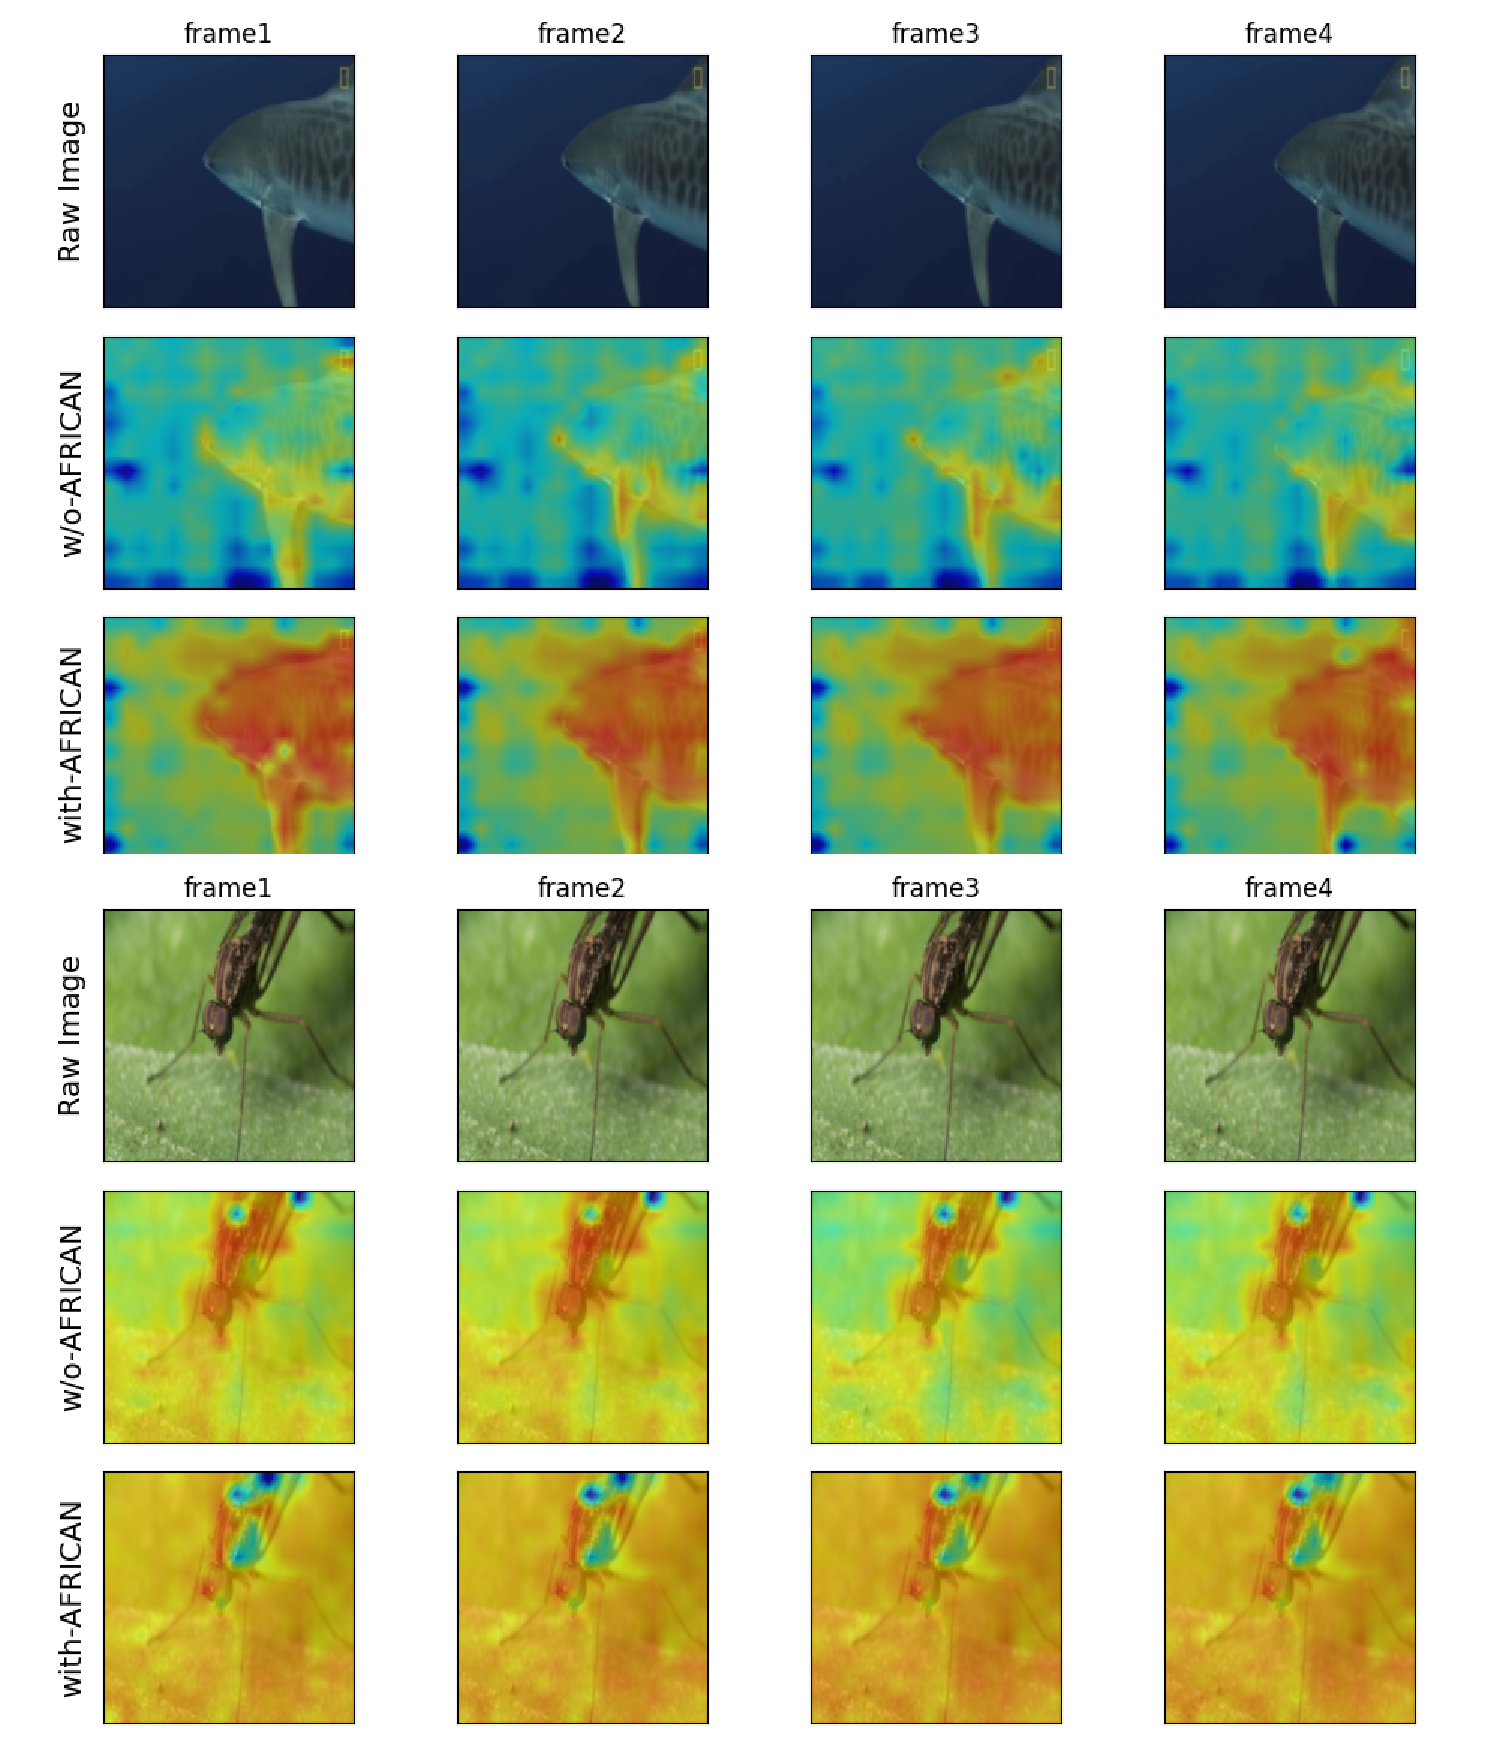
\includegraphics[width=0.9\textwidth]{assets/charts/4_5_AttentionMaps_1}
    \caption[Attention Map 1 (Good examples)]{The examples of attention map on two videos that with-AFRICAN outperform w/o-AFRICAN. The first row is the input video, the second row is the attention map of w/o-AFRICAN, and the third row is the attention map of with-AFRICAN. w/o-AFRICAN represents the CLIP model without AFRICAN pretraining, while with-AFRICAN represents the CLIP model with AFRICAN pretraining.}
    \label{fig:attnmap1}
\end{figure}

% \begin{figure}[ht]
%     \centering
%     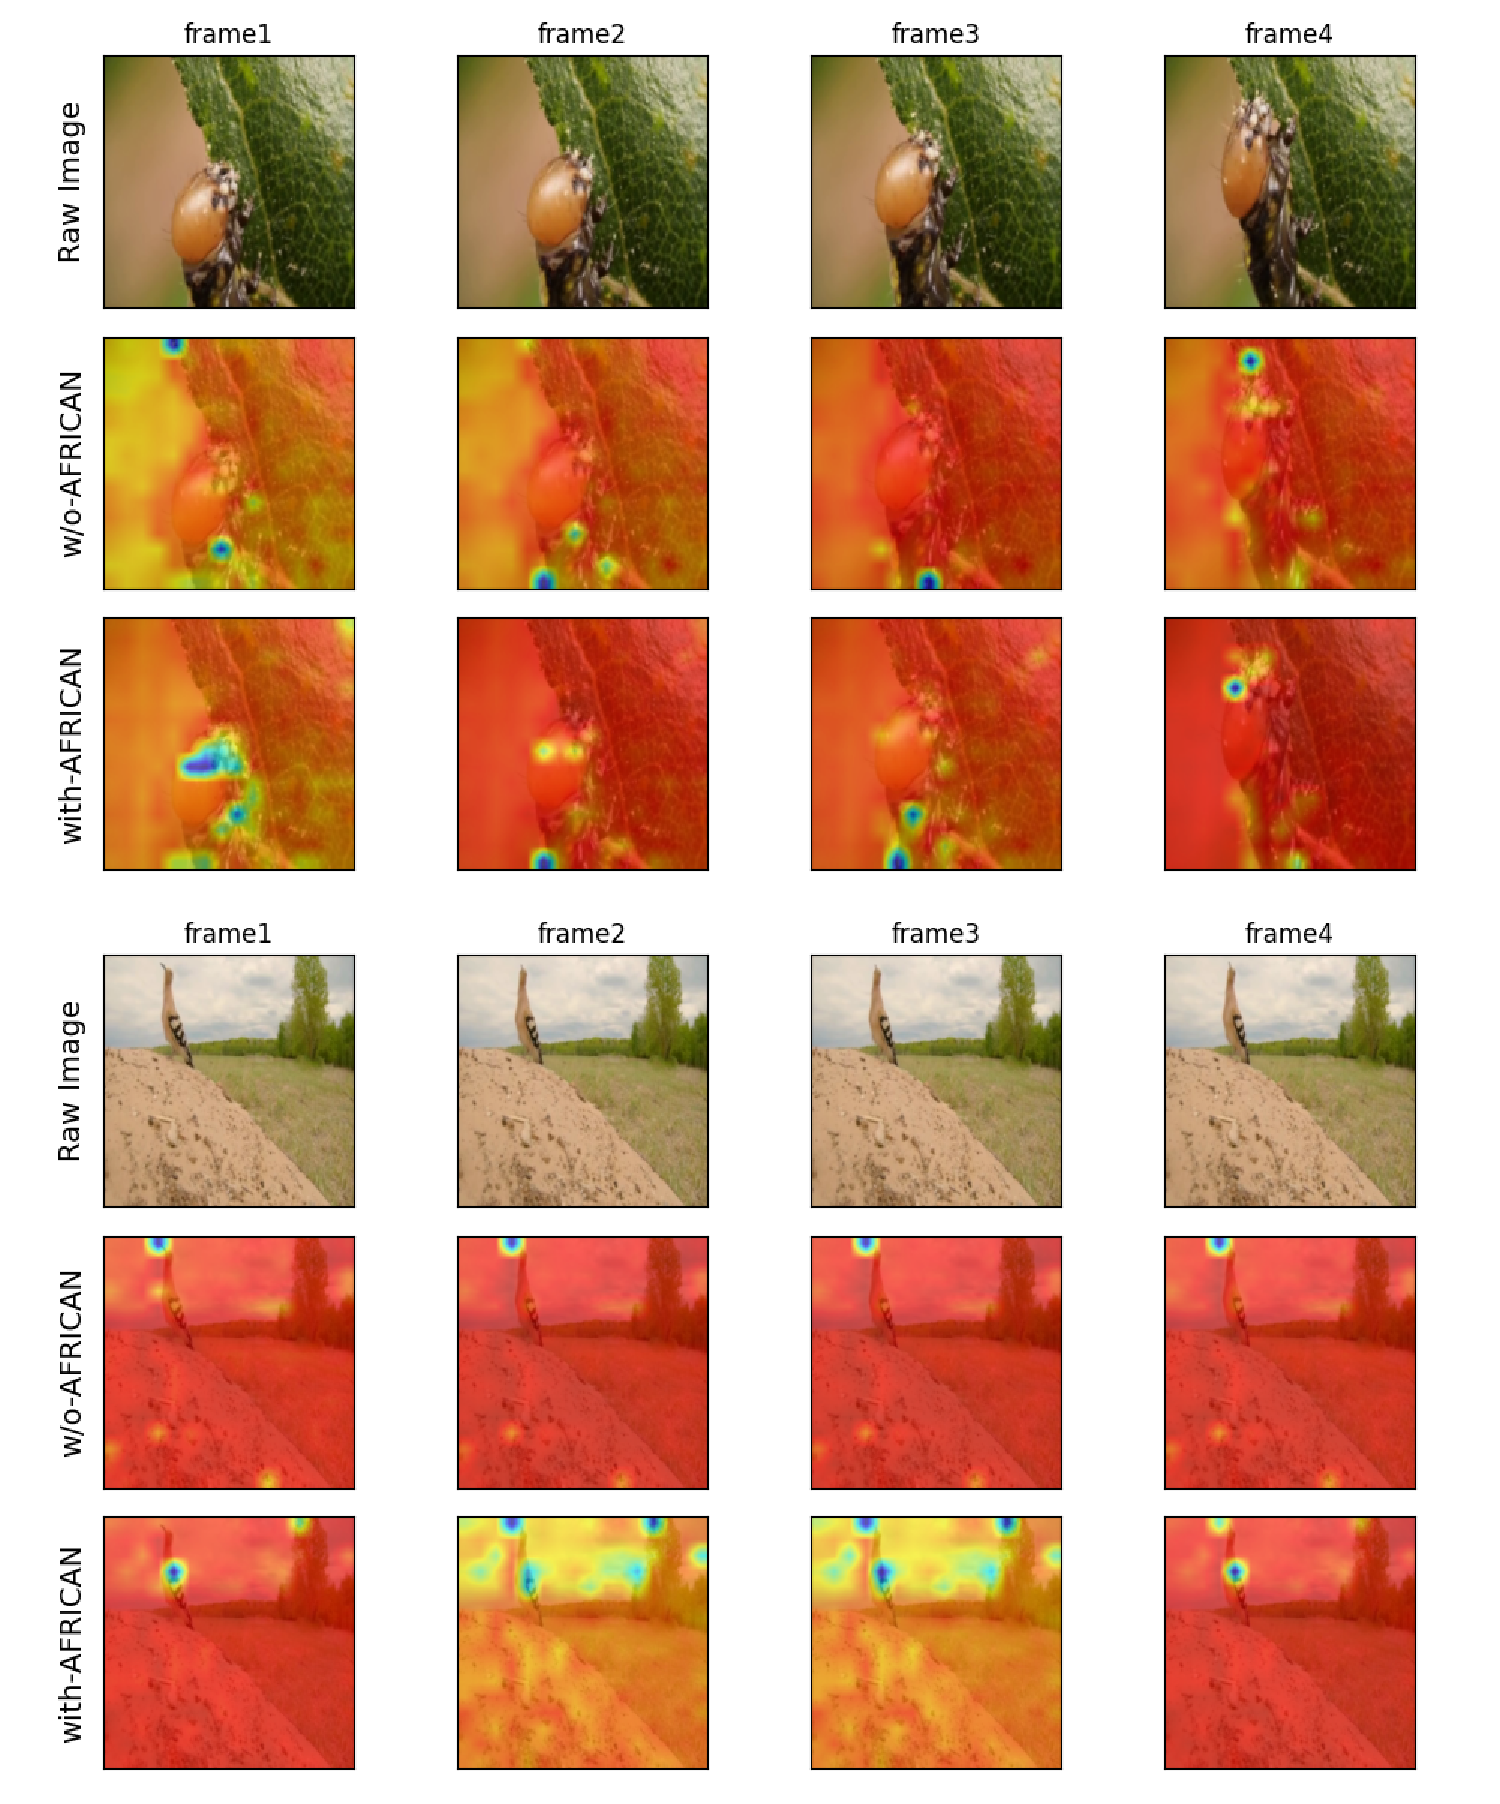
\includegraphics[width=1.0\textwidth]{assets/charts/4_5_AttentionMaps_2}
%     \caption[Attention Map 2 (Good examples)]{The same as Figure \ref{fig:attnmap1} on another two videos.}
%     \label{fig:attnmap2}
% \end{figure}

\begin{figure}[ht]
    \centering
    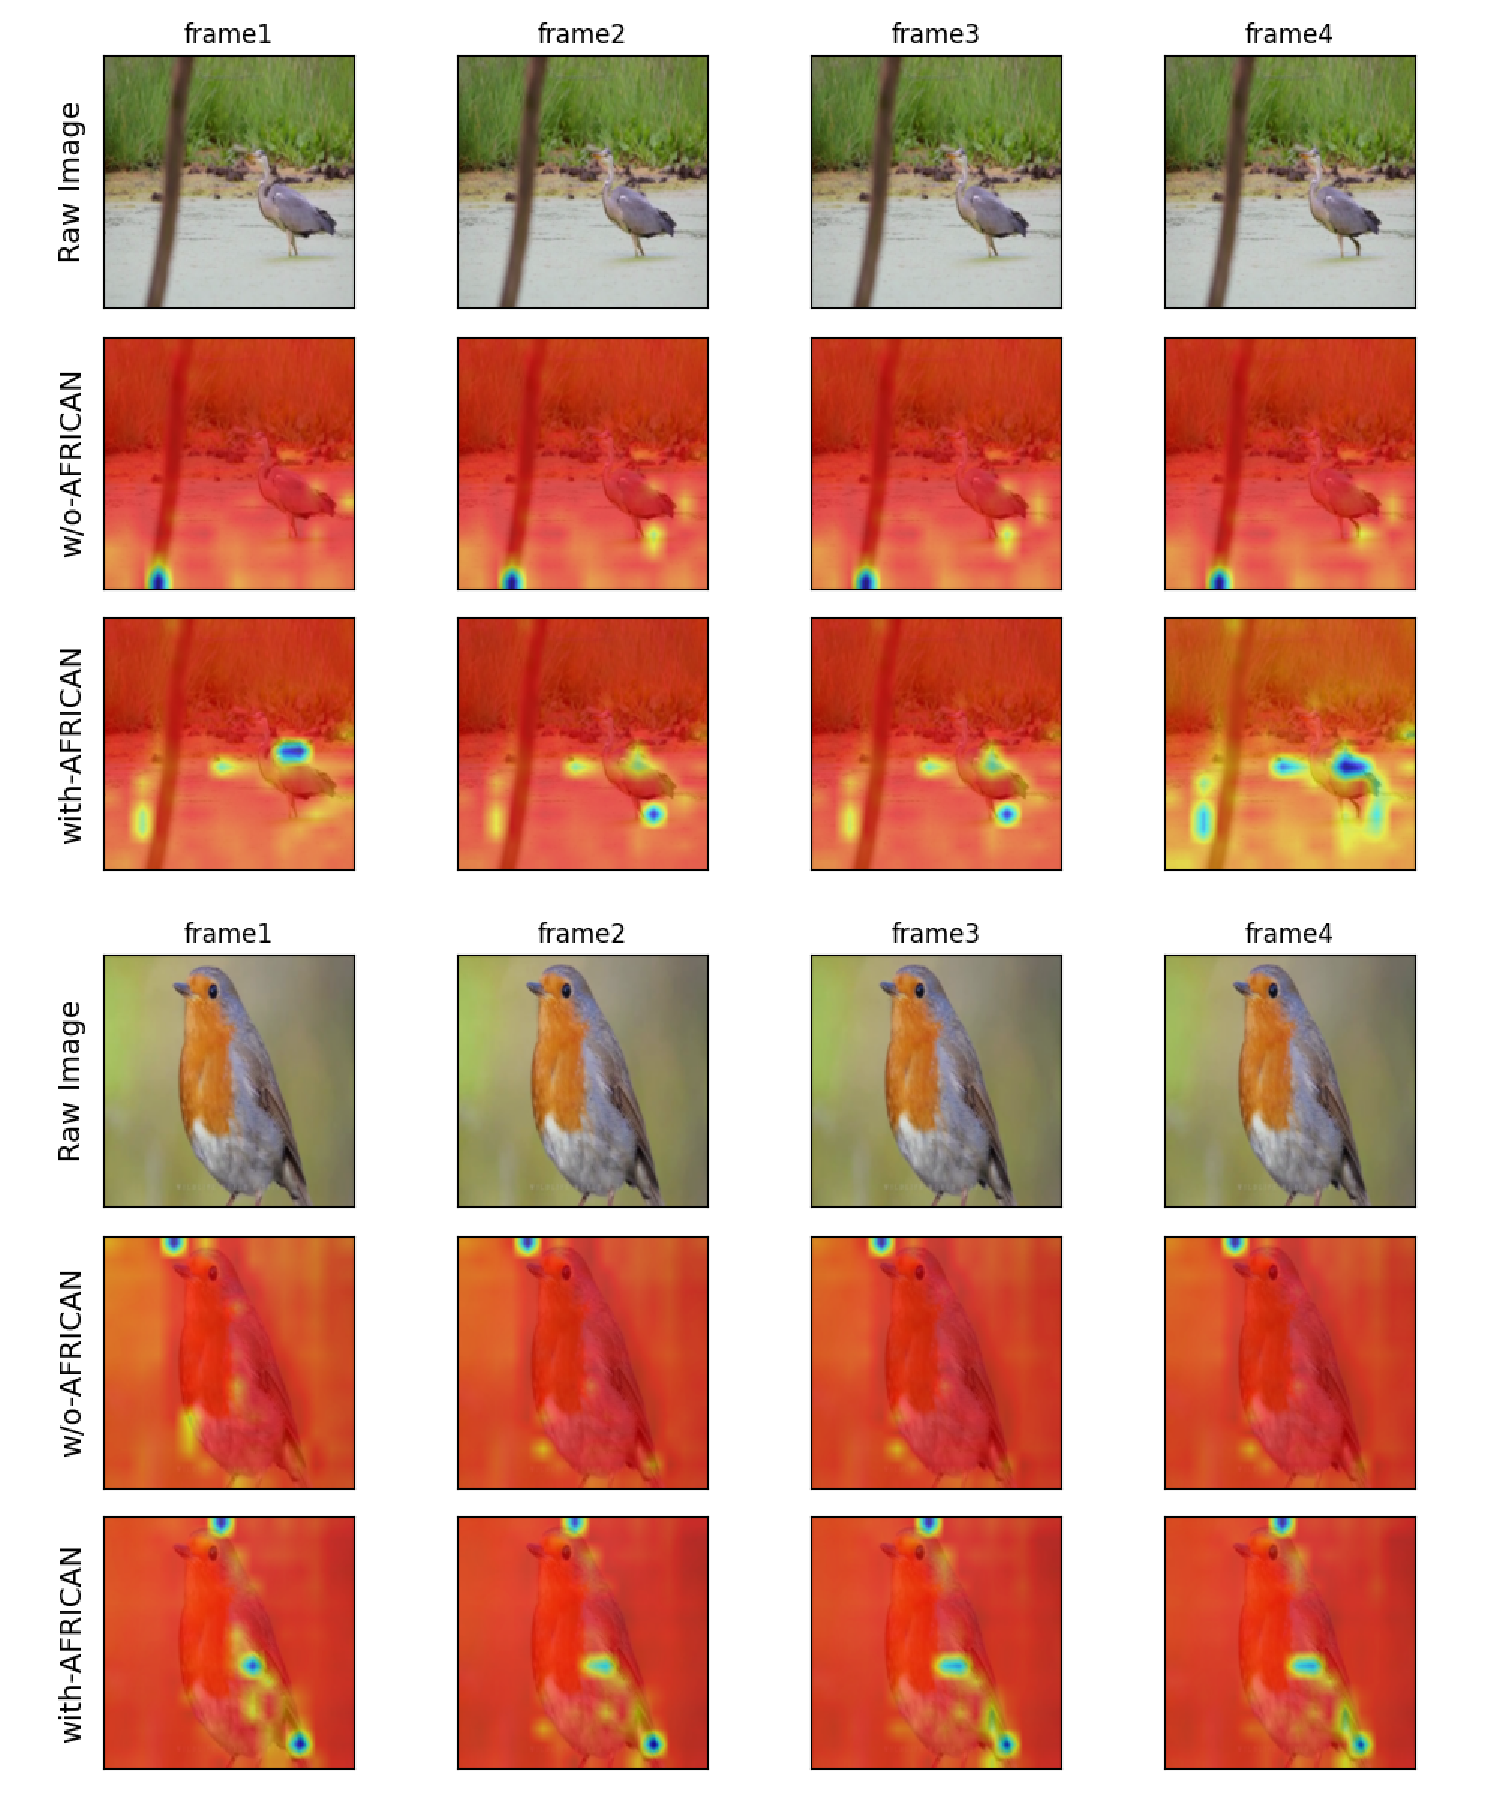
\includegraphics[width=0.9\textwidth]{assets/charts/4_5_AttentionMaps_3}
    \caption[Attention Map 3 (Good examples)]{The same as Figure \ref{fig:attnmap1} on another two videos.}
    \label{fig:attnmap3}
\end{figure}

\begin{figure}[ht]
    \centering
    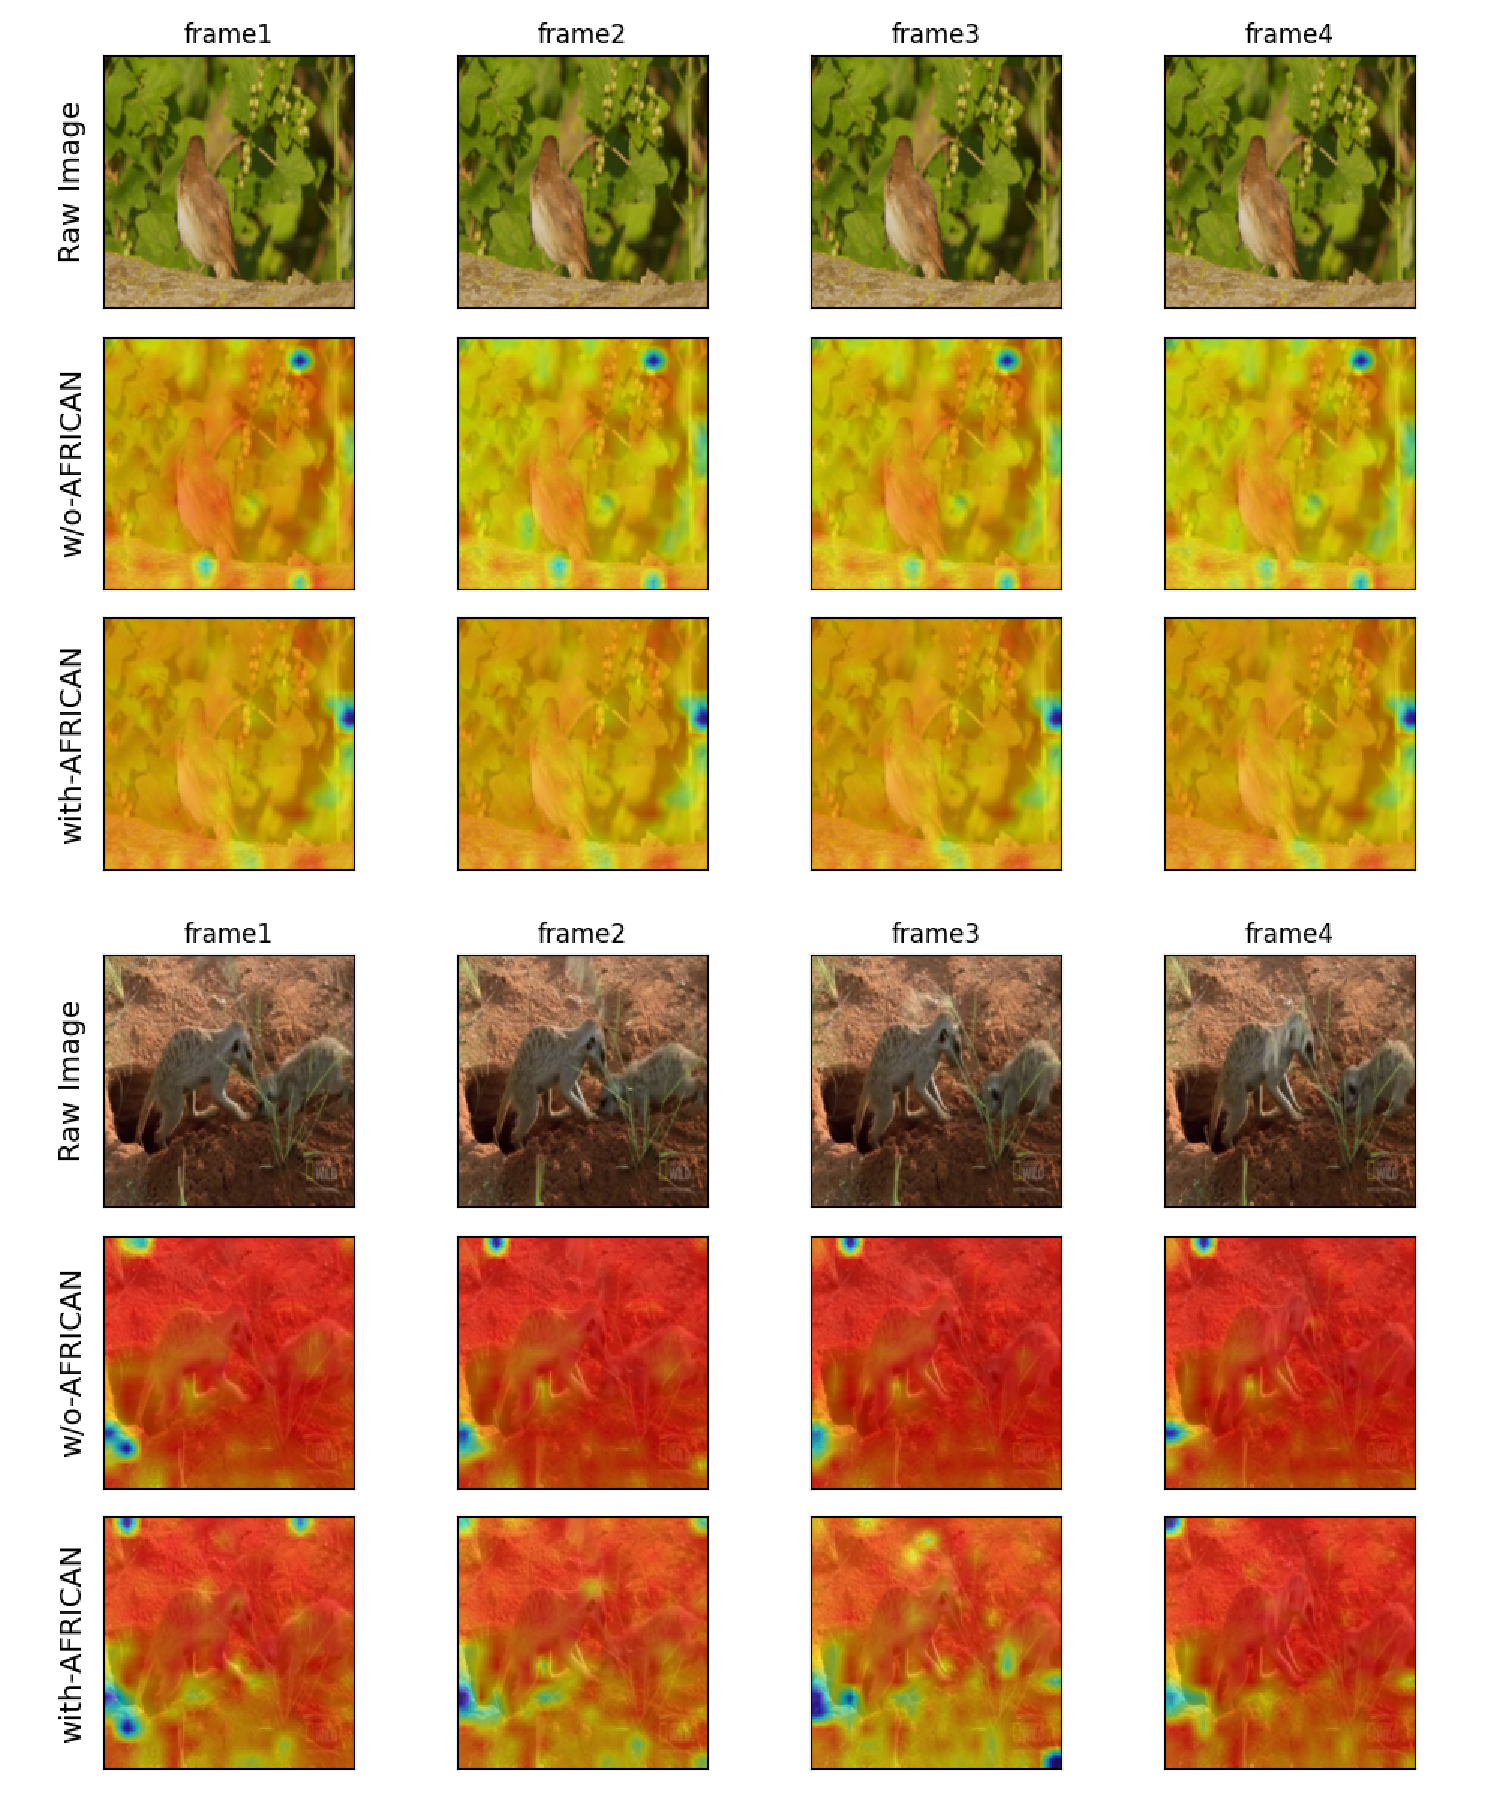
\includegraphics[width=0.9\textwidth]{assets/charts/4_5_AttentionMaps_4}
    \caption[Attention Map 4 (Bad examples)]{The examples of attention map on two videos that both model does not perform well. The first row is the input video, the second row is the attention map of w/o-AFRICAN, and the third row is the attention map of with-AFRICAN. w/o-AFRICAN represents the CLIP model without AFRICAN pretraining, while with-AFRICAN represents the CLIP model with AFRICAN pretraining.}
    \label{fig:attnmap4}
\end{figure}




\subsection{Action Recognition Stage}
The AFRICAN model for action recognition, denoted as AFRICAN-AR, is illustrated in Figure \ref{fig:modelstructaf_ar}. This model is trained with a Focal Loss and the adamw optimizer using a learning rate of 0.00015 on a single A100 GPU. As the VideoCLIP module of InterVideo takes longer to converge illustrated in Figure \ref{fig:tp_backbone} where the IC model does not improve after 40 epochs, all models in this experiment are trained for 40 epochs. The mAP is used as the evaluation metric for this task.

Figure \ref{fig:final_result} illustrates the performance of IC and AFRICAN-AR. It is obvious that AFRICAN-AR outperforms in the Head and Middle classes, but performs equally with the IC in the Tail classes. Considering the larger variance of performance of IC in tail classes, Epoch 40, where they have very close mAP in tail classes, is picked to evaluate the two models fairly. 

The results for action recognition at Epoch 40 are presented in Table \ref{tab:allresults40}. With the stream of pretrained AFRICAN weights, AFRICAN-AR is able to improve IC model with 1.82\% (from 52.48\% to 54.30\%) overall mAP with the majority improvement on the head and middle classes.

\begin{figure}
    \centering
    \begin{adjustwidth}{-0.15\linewidth}{-0.07\linewidth}
    \begin{subfigure}[b]{0.65\textwidth}
        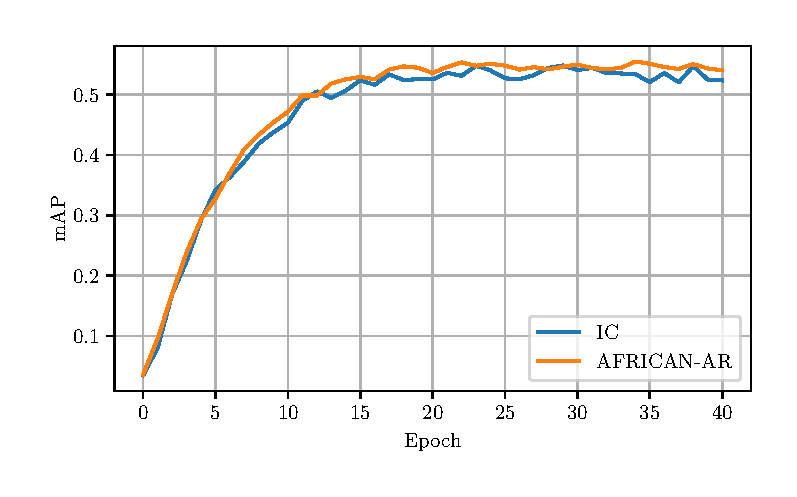
\includegraphics[width=\textwidth]{assets/charts/4_4_finalscore_0_overall}
        \caption{Overall Performance}
        \label{fig:subfig1}
    \end{subfigure}
    \begin{subfigure}[b]{0.65\textwidth}
        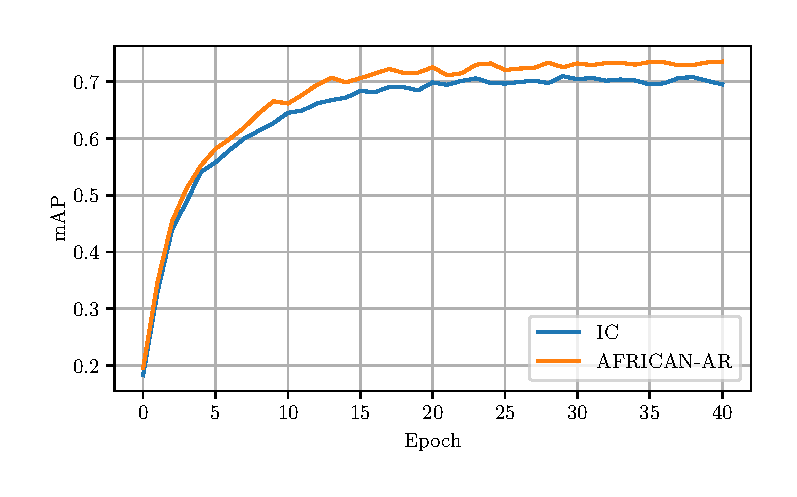
\includegraphics[width=\textwidth]{assets/charts/4_4_finalscore_1_head}
        \caption{Head Classes Performance}
        \label{fig:subfig2}
    \end{subfigure}

    \vspace{10pt} % Adjust the spacing as needed

    \begin{subfigure}[b]{0.65\textwidth}
        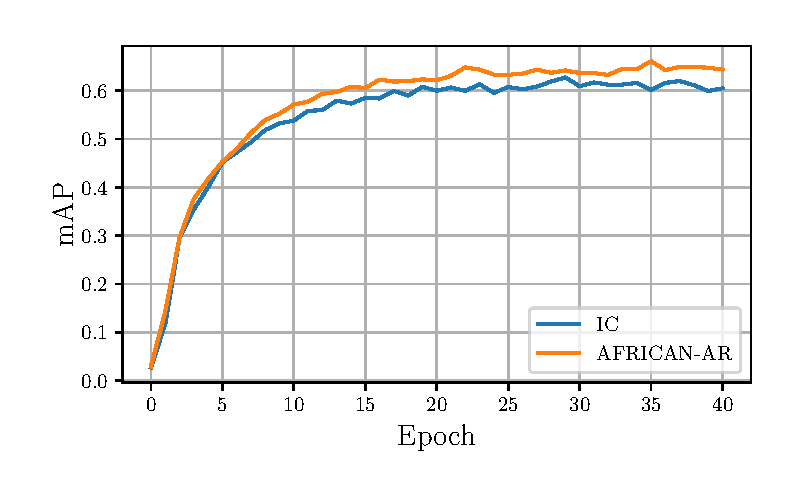
\includegraphics[width=\textwidth]{assets/charts/4_4_finalscore_2_middle}
        \caption{Middle Classes Performance}
        \label{fig:subfig3}
    \end{subfigure}
    \begin{subfigure}[b]{0.65\textwidth}
        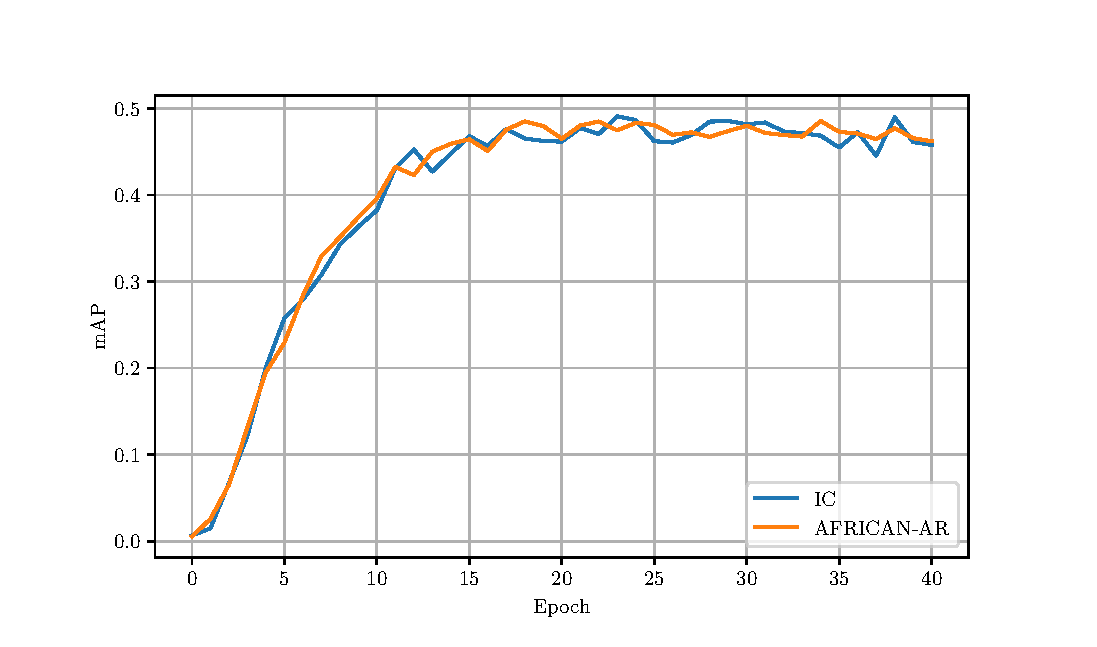
\includegraphics[width=\textwidth]{assets/charts/4_4_finalscore_3_tail}
        \caption{Tail Classes Performance}
        \label{fig:subfig4}
    \end{subfigure}
    \caption[The Performance of IC and AFRICAN-AR on each Epoch for Different Segments]{This figure illustrates The Performance of IC and AFRICAN-AR on each Epoch for Different Segments. \textbf{IC} represents ImageCLIP trained on post-transformer layers, as illustrated in Figure \ref{fig:modelstructure_ic} with a frozen image encoder, while \textbf{AFRICAN-AR} use the same structure as IC but with AFRICAN pretrained weights, as illustrated in Figure \ref{fig:modelstructaf_ar}}
    \label{fig:final_result}
    
\end{adjustwidth}
\end{figure}



\begin{table}[ht]
    \centering
    \caption[Results of action recognition (Epoch 40)]{The Table shows the results of action recognition on Epoch 40. \textbf{IC} represents ImageCLIP trained on post-transformer layers, as illustrated in Figure \ref{fig:modelstructure_ic} with a frozen image encoder, while \textbf{AFRICAN-AR} uses the same structure as IC but with AFRICAN pretrained weights, as illustrated in Figure \ref{fig:modelstructaf_ar}}
    \label{tab:allresults40}
    \begin{tabular}{lllll}
        \toprule
        \multirow{2}{*}{Models} & \multicolumn{4}{c}{mAP (Epoch 40)} \\
        \cmidrule{2-5} 
        {} & Overall & Head  & Middle & Tail \\
        \midrule
        IC            & 52.48   & 69.53 & 60.52 & 45.79 \\        
        AFRICAN-AR    & \textbf{54.30} & \textbf{73.54} & \textbf{64.38} & \textbf{46.21} \\
        \bottomrule
    \end{tabular}
\end{table}


\section{Final Result}
To fairly compare AFRICAN-AR and IC with the baseline model, CARe, Table \ref{tab:allresultsbest} displays the best result of the CARe, IC (Epoch 29), AFRICAN-AR (Epoch 34), and MSQNet. It is evident that AFRICAN-AR consistently outperforms CARe across all segments, with 24.90\% overall mAP improvement, 9.66\% improvement in head classes, 25.84\% improvement in middle classes, and 23.45\% improvement in tail classes, enabling it to achieve its best score of 55.45\% mAP. The comparison with the state-of-the-art model, MSQNet, will be discussed in the section \ref{sec:discussion_msqnet}

\begin{table}[ht]
    \centering
    \caption[Results of action recognition (Best Epoch)]{The table shows the results of CARe, IC, AFRICAN-AR, and MSQNet for action recognition. \textbf{CARe} is proposed by Animal Kingdom \parencite{ng2022animal} and used as the baseline model in this research. \textbf{IC} represents ImageCLIP trained on post-transformer layers, as illustrated in Figure \ref{fig:modelstructure_ic} with a frozen image encoder. \textbf{AFRICAN-AR} uses the same structure as IC but with AFRICAN pretrained weights, as illustrated in Figure \ref{fig:modelstructaf_ar}. \textbf{MSQNet} is the state-of-the-art model for action recognition on the Animal Kingdom dataset.}
    \label{tab:allresultsbest}
    
    \begin{tabular}{lllll}
        \toprule
        \multirow{2}{*}{Models} & \multicolumn{4}{c}{mAP (Best Epoch)} \\
        \cmidrule{2-5} 
        {} & Overall & Head  & Middle & Tail \\
        \midrule
        CARe\parencite{ng2022animal}       & 30.55          & 63.33          & 38.62          & 25.09 \\
        IC                                 & 54.79          & \uuline{70.18} & \uuline{62.76} & \textbf{48.54} \\
        AFRICAN-AR                         & \uuline{55.45} & \textbf{72.99} & \textbf{64.46} & \textbf{48.54} \\
        MSQNet\parencite{mondal2023msqnet} & \textbf{67.74}   &  -    & -     & - \\ 
        \bottomrule
    \end{tabular}
\end{table}

